\documentclass[11pt]{article}
\usepackage[spanish]{babel}
\usepackage[utf8x]{inputenc}
\usepackage{amsmath,amssymb, amsthm}
\usepackage{graphicx}
\usepackage{subfigure}
\usepackage{url}
\usepackage{float}
\usepackage{multicol}
\usepackage{multirow}
\spanishdecimal{.}
\usepackage{fullpage}
\usepackage{enumerate}
\usepackage{enumitem}
\usepackage[table]{xcolor}
\graphicspath{{figuras/}}


\usepackage{listings}
\usepackage{color}
\definecolor{brown}{rgb}{0.48, 0.25, 0.0}
\definecolor{codegray}{rgb}{0.5,0.5,0.5}
\definecolor{backcolour}{rgb}{0.95,0.95,0.92}
 
\lstdefinestyle{mystyle}{
    backgroundcolor=\color{backcolour},   
    commentstyle=\color{blue},
    keywordstyle=\color{brown},
    numberstyle=\tiny\color{codegray},
    stringstyle=\color{magenta},
    basicstyle=\footnotesize,
    breakatwhitespace=false,         
    breaklines=true,                                  
    keepspaces=true,                 
    numbers=left,                    
    numbersep=5pt,                  
    showspaces=false,                
    showstringspaces=false,
    showtabs=false,                  
    tabsize=8,
    frame=single,
}
 
\lstset{style=mystyle}
\renewcommand{\lstlistingname}{Algoritmo}% Listing -> Algorithm

\newtheorem{innercustomgeneric}{\customgenericname}
\providecommand{\customgenericname}{}
\newcommand{\newcustomtheorem}[2]{%
  \newenvironment{#1}[1]
  {%
   \renewcommand\customgenericname{#2}%
   \renewcommand\theinnercustomgeneric{##1}%
   \innercustomgeneric
  }
  {\endinnercustomgeneric}
}

\newcustomtheorem{customtheorem}{Teorema}


\title{Proyecto Instrumentación}
\author{Herrera Alcantar Hiram Kalid}

\begin{document}
\begin{titlepage}
\begin{center}
\Huge Universidad Autónoma de Baja California
\huge Facultad de Ciencias
\vspace{0.8cm}
\begin{figure}[H]
\centering

\includegraphics[width=0.3\textwidth]{uabc}
\end{figure}
\huge Proyecto de Instrumentación\\
\huge\textbf{{GENERADOR DE FUNCIONES}}

\vspace{1.5cm}
\Huge{Hiram K. Herrera Alcantar \\ Osvaldo Rosales Pérez}

\vspace{1.5cm}
\huge{Profesor:}\\
\huge Dra. Eloisa del Carmen García Canseco \\
\vspace{1.5cm}
\LARGE Fecha: 26 de Mayo del 2017
\end{center}
\end{titlepage}
\newpage
\section{Objetivo}
Desarrollar un generador de funciones aplicando conocimientos de electrónica adquiridos en la clase de instrumentación y conocimientos de previos de programación.
\section{Introducción}
Un generador de funciones generalmente es un equipo o software de prueba, usado para generar diferentes tipos de formas de ondas eléctricas en un rango de frecuencias establecido. Típicamente las formas de onda disponibles en un generador de funciones son la senoidal, cuadrada, triangular y diente de sierra; que pueden ser repetitivas o singulares. En general un generador de funciones se utiliza para examinar y reparar circuitos electrónicos, aunque también pueden ser utilizados para calibrar equipos, rampas de alimentación, etc \cite{klaassen1996electronic}.

El propósito de este proyecto es construir un generador de funciones sencillo,tomando como base el que se presenta en \cite{amandaghassaei}; y utilizando herramientas de electrónica y programación, para esto se implementa un microcontrolador Arduino UNO en la realización del proyecto, además de diversos componentes electrónicos que se describirán más adelante. Como aportación al modelo de un generador se agrega una modulación por ancho de pulsos (PWM), que se encarga de modificar el ancho de los pulsos cuadrados.

Cabe mencionar la importancia de la instrumentación en la realización de este proyecto, pues al hacer las conexiones es necesario comprobar el valor de la corriente y voltaje que corre sobre cada componente pues de lo contrario podrían dañarse; además se debe comprobar continuidad de corriente, para esto se utiliza un multímetro. Otro punto importante de la instrumentación en este proyecto es el uso del osciloscopio para desplegar las formas de onda generadas por el dispositivo.



\section{Materiales}
\begin{multicols}{2}
\begin{itemize}
\item 4 Pushbutton de 4 pines.
\item 12 resistores de 10k Ohm.
\item 9 resistores de 20k Ohm.
\item 1 resistores de 2.2k Ohm
\item 4 resistores de 1k ohm. 
\item 1 Potenciometro de 50k Ohm.
\item 2 Potenciometros de 10k Ohm.
\item 2 Capacitores electrolíticos de 220$\mu$F.
\item Circuito integrado LM386N.
\item Batería de 9V.
\item 4 diodos LED.
\item Protoboard.
\item Arduino UNO.
\item Cable UTP.
\end{itemize}
\end{multicols}

\section{Funcionamiento electrónico}
El generador de funciones se basa principalmente en el Arduino UNO para el cálculo y la generación de cada función. Sin embargo, sigue siendo necesario un circuito externo para manejar las señales de entrada y salida del microcontrolador. Este circuito externo consta de 4 secciones, una de entradas, otra de salidas, un convertidor digital-analógico y un amplificación de señal.


\subsection*{Entradas}
Las entradas que se tienen son los cuatro botones push que sirven para seleccionar el tipo de función a generar, ya sea sinusoidal, sierra, triangular o cuadrada. También están los potenciómetros, dos de éstos fijan la frecuencia de las funciones y, en caso de seleccionar la función cuadrada, el ancho de cada pulso. El tercer potenciómetro controla la ganancia o amplitud de las funciones.


\subsection*{Salidas}
Se tienen cuatro salidas para LEDs, cada uno corresponde a una función del generador y se encienden la momento de hacer la selección con los interruptores de entrada. También se tiene la salida digital que abarca 8 pines (D0-D7), la cual se encarga de transmitir la señal de la función seleccionada al convertidor digital-analógico.


\subsection*{Convertidor digital analógico (DAC)}
Éste se encarga de tomar la señal digital de salida del Arduino en la que se transmite el valor de la función y la transforma a una señal analógica.

\noindent El convertidor utilizado es uno del tipo escalera R-2R, el cual se basa en arreglos repetitivos de resistencias en una configuración de escalera, como se muestra en la figura \ref{fig:DAC_diagram}.

\begin{figure}[htb]
\centering
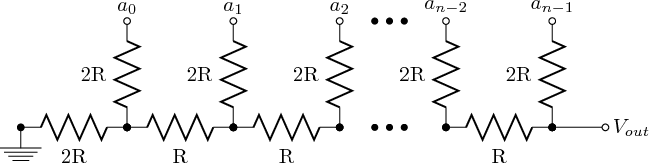
\includegraphics[width = 0.55\textwidth]{R2r-ladder.png}
\caption{Convertidor digital-analógico con $n$ entradas digitales $a_0,...,a_{n-1}$ y salida analógica $V_{out}$}
\label{fig:DAC_diagram}
\end{figure}

\noindent Este arreglo R-2R hace que cada bit sea pesado por su contribución al voltaje de salida $V_{out}$. Dependiendo de cuales bits son $1$ o $0$, el voltaje de salida tendrá el correspondiente valor entre $0V$ y $V_{ref}=5V$.


\subsection*{Amplificador de señal}
La sección del amplificador de señal sirve para que una vez obtenida una señal analógica del DAC, ésta se amplifique, pues generalmente en el proceso de conversión se pierde energía además de que las salidas del Arduino solo pueden proporcionar como máximo 5V.
Para lograr la amplificación de la señal se implementó un amplificador operacional, particularmente, el circuito integrado LM386n.

El diseño general de un amplificador operacional se muestra en la figura \ref{fig:Op-amp} donde $V_+$ y $V_-$ corresponden a la señal de entrada, $V_{S+}$ y $V_{S-}$ son la diferencia de potencial que establece el rango de amplificación y $V_{out}$ es la señal ya amplificada.

\begin{figure}[H]
\centering
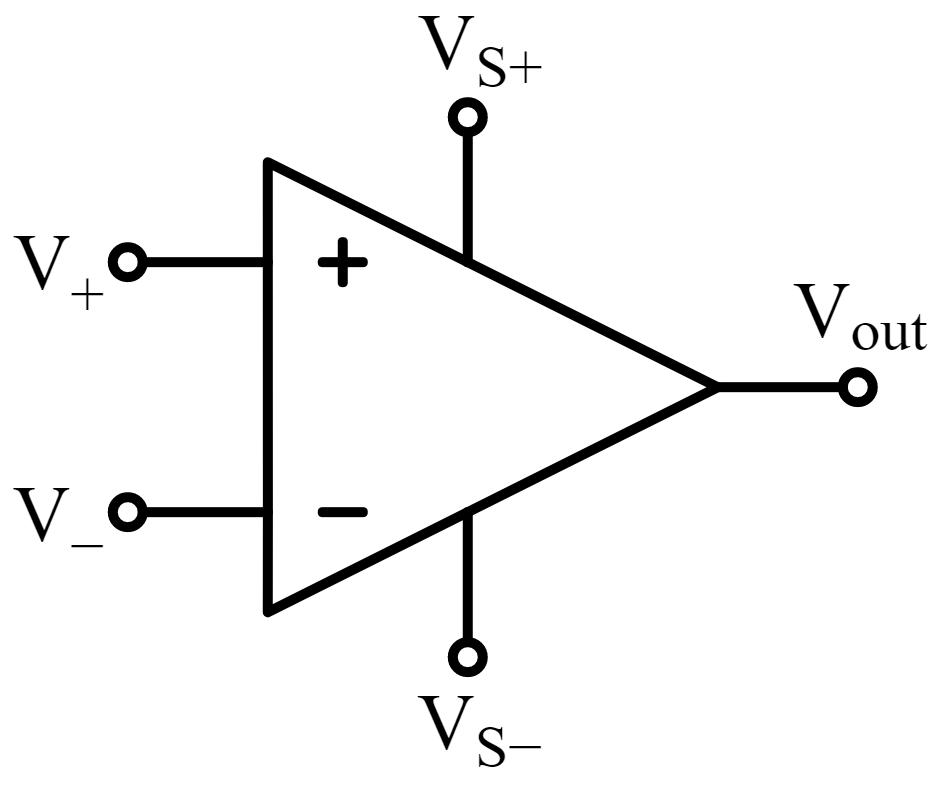
\includegraphics[width = 0.19\textwidth]{Op-amp.PNG}
\caption{Amplificador operacional.}
\label{fig:Op-amp}
\end{figure}


\section{Funcionamiento general}
La operación del generador de funciones es bastante simple. Como se muestra en la figura \ref{fig:Operacion}, en necesario alimentar el generador con 9V (terminales caimán rojo y negro), ya sea de una fuente de voltaje o una batería. Los 9V van al amplificador y al Arduino, todos los demás componentes trabajan con 5V suministrados por el mismo Arduino. La función generada, una vez amplificada, se puede medir en el pin central del potenciómetro de ganancia, conectado a la salida del amplificador. La conexión con el osciloscopio es con la sonda de prueba conectada a éste pin y la otra terminal conectada a la tierra de la fuente de alimentación.

Una vez que se conecta el circuito a la fuente de alimentación y la sonda del osciloscopio se conecta al potenciometro de ganancia, es posible controlar la función generada y ver los cambios en la pantalla del osciloscopio.

La selección del tipo de señal es con los botones en el centro del protoboard. De los tres potenciómetros colocados en el extremo izquierdo del circuito, el primero, de izquierda a derecha, controla la amplitud de la señal, el siguiente controla la frecuencia y el último controla el ancho de los pulsos cuadrados.

La amplitud máxima para una señal es de 7V. El rango dinámico de frecuencias es de $300-15,000Hz$ para las señales sinusoidal, sierra y triangular, mientras que la señal cuadrada puede trabajar en el rango de $300-25,000Hz$.

En la figura \ref{fig:results} se pueden ver los 4 tipos de señal que se pueden generar ademas de la modulación de ancho de pulso para las ondas cuadradas.

\begin{figure}[H]
\centering
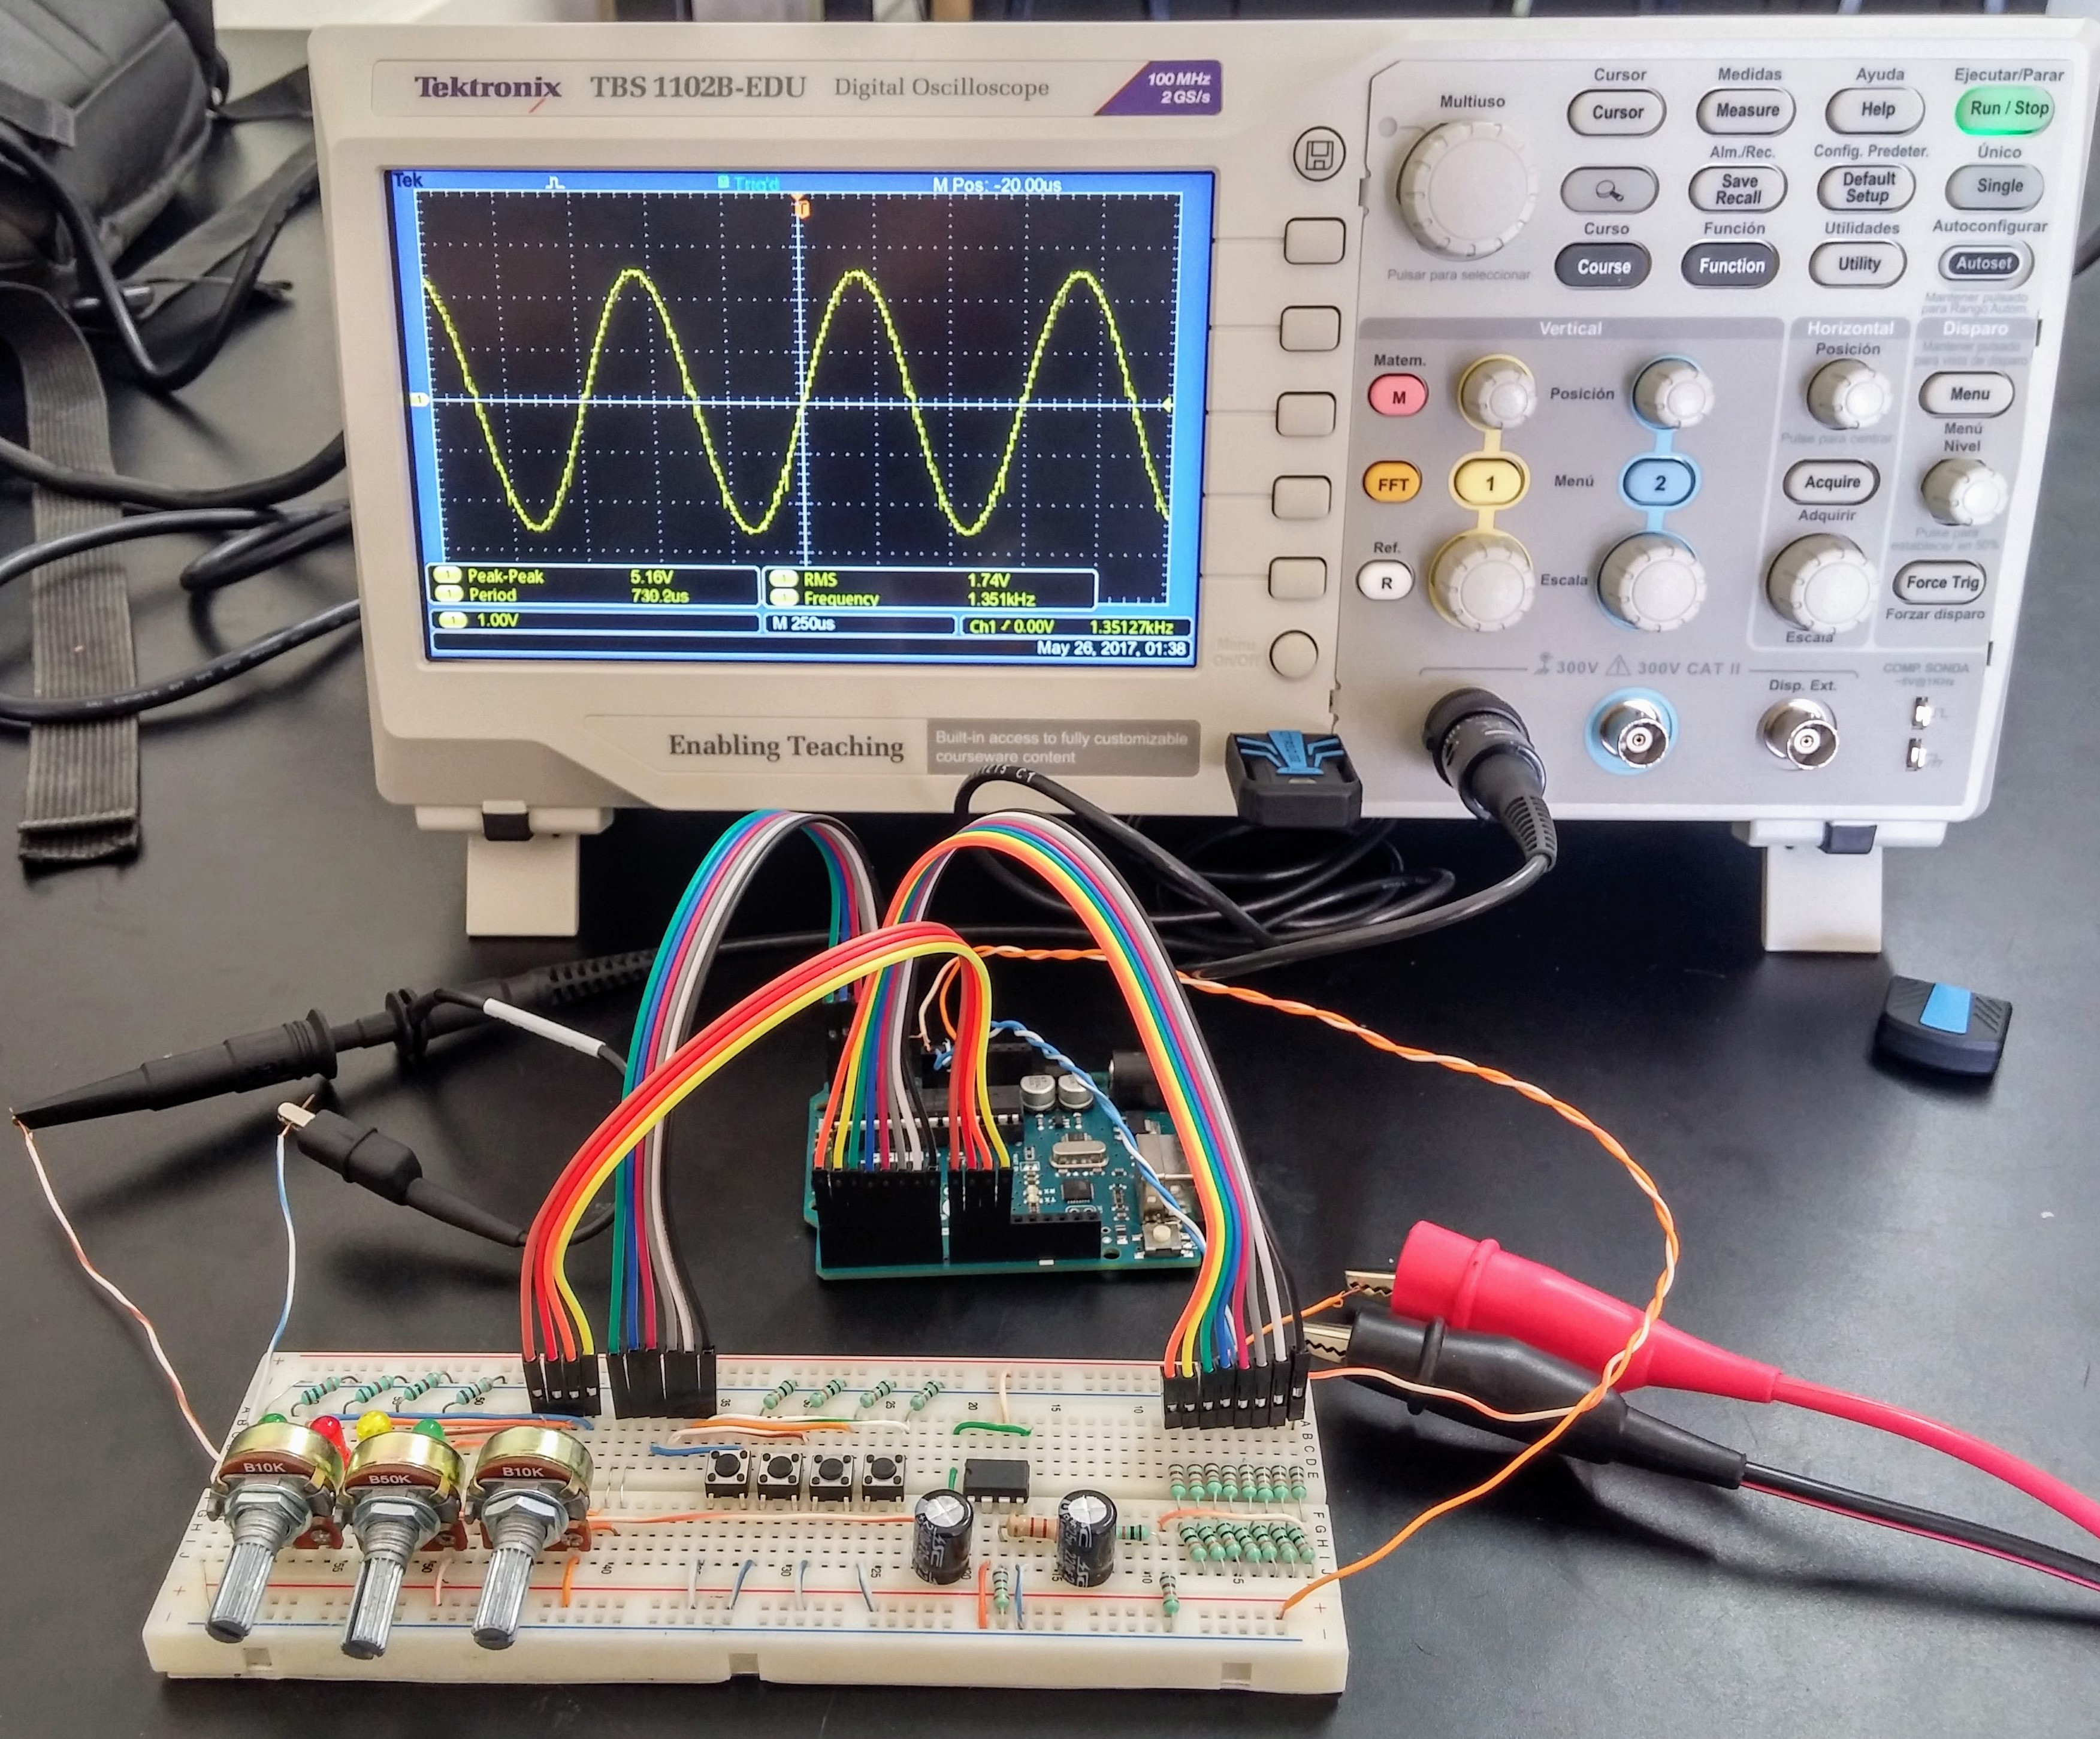
\includegraphics[width = 0.45\textwidth]{Operacion.jpg}
\caption{Generador de funcione en operación}
\label{fig:Operacion}
\end{figure}

\begin{figure}[htb]
\centering
\subfigure[Pulso]{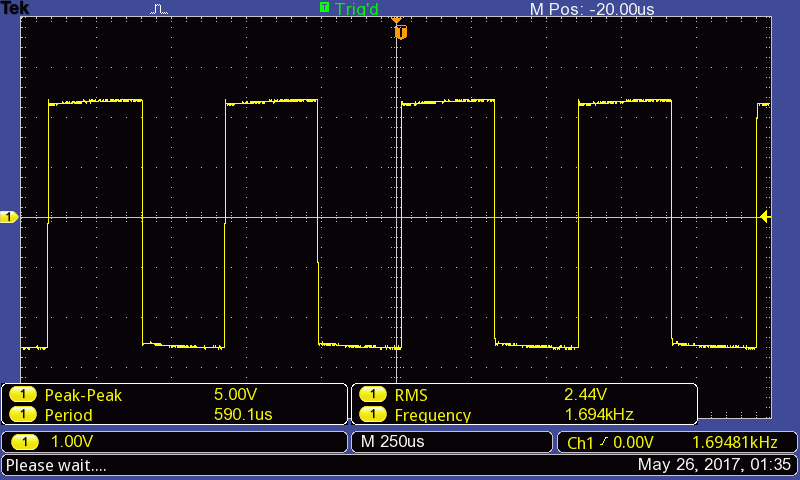
\includegraphics[width = 0.37\textwidth]{Pulse}}
\subfigure[Pulso con ancho modulado]{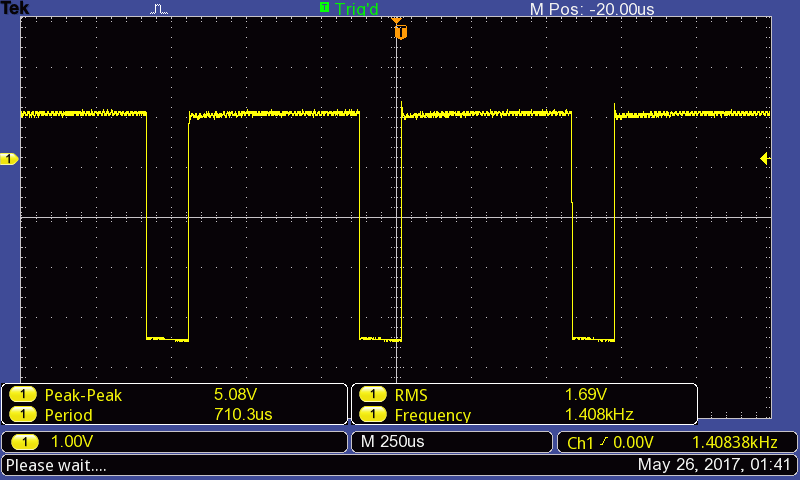
\includegraphics[width = 0.37\textwidth]{Pulse_mod}}
\subfigure[Sierra]{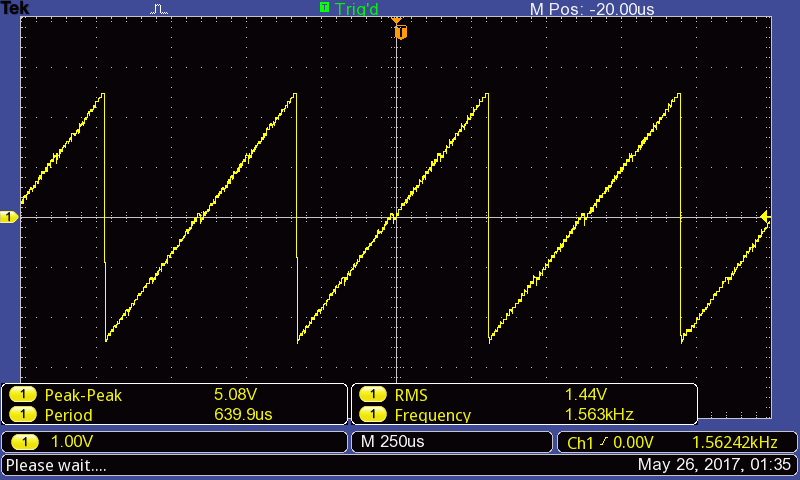
\includegraphics[width = 0.37\textwidth]{Saw}}
\subfigure[Triangular]{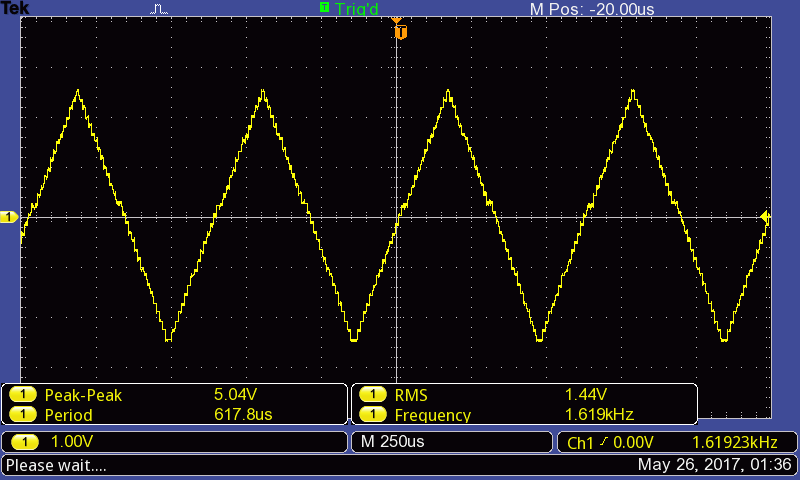
\includegraphics[width = 0.37\textwidth]{Triangular}}
\subfigure[Seno]{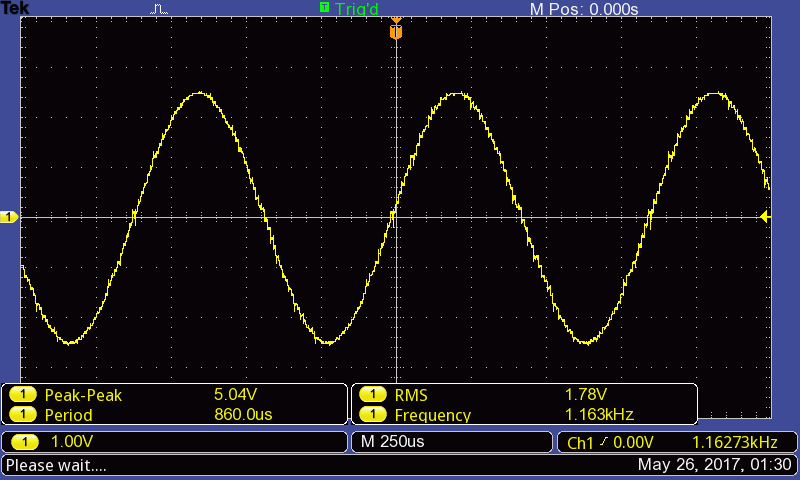
\includegraphics[width = 0.37\textwidth]{Sine}}
\caption{Resultados obtenidos.}
\label{fig:results}
\end{figure}


\section{Desarrollo del proyecto.}
El procedimiento para el ensamblado del dispositivo se describe a continuación
\begin{enumerate}[label=\textbf{Paso \arabic*:}]
\item \textbf{Instalación de botones.}\\
Se conectan los cuatro botones al protoboard tal como se muestra en la figura \ref{fig:pushbutton}, éstos se conectan a tierra y a la salida de 5V del Arduino a través de un resistor de 10k Ohms cada uno. Entre cada botón y tierra se hace una conexión hacia las entradas analogicas A0-A3 del Arduino. Se conectan en el  siguiente orden: 
\begin{itemize}
\item A0 = Pulso
\item A1 = Triangulo
\item A2 = Sierra
\item A3 = Seno
\end{itemize}

\begin{figure}[htb]
\centering
\subfigure[Diagrama]{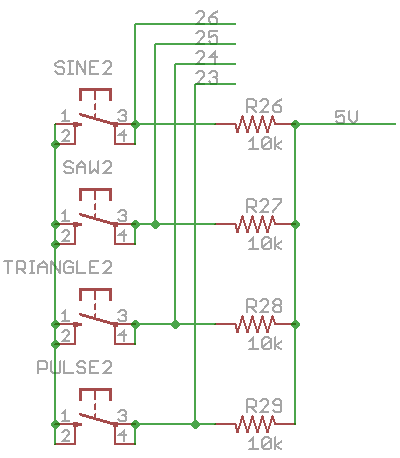
\includegraphics[width = 0.25\textwidth]{botones}}
\subfigure[Ensamble en protoboard]{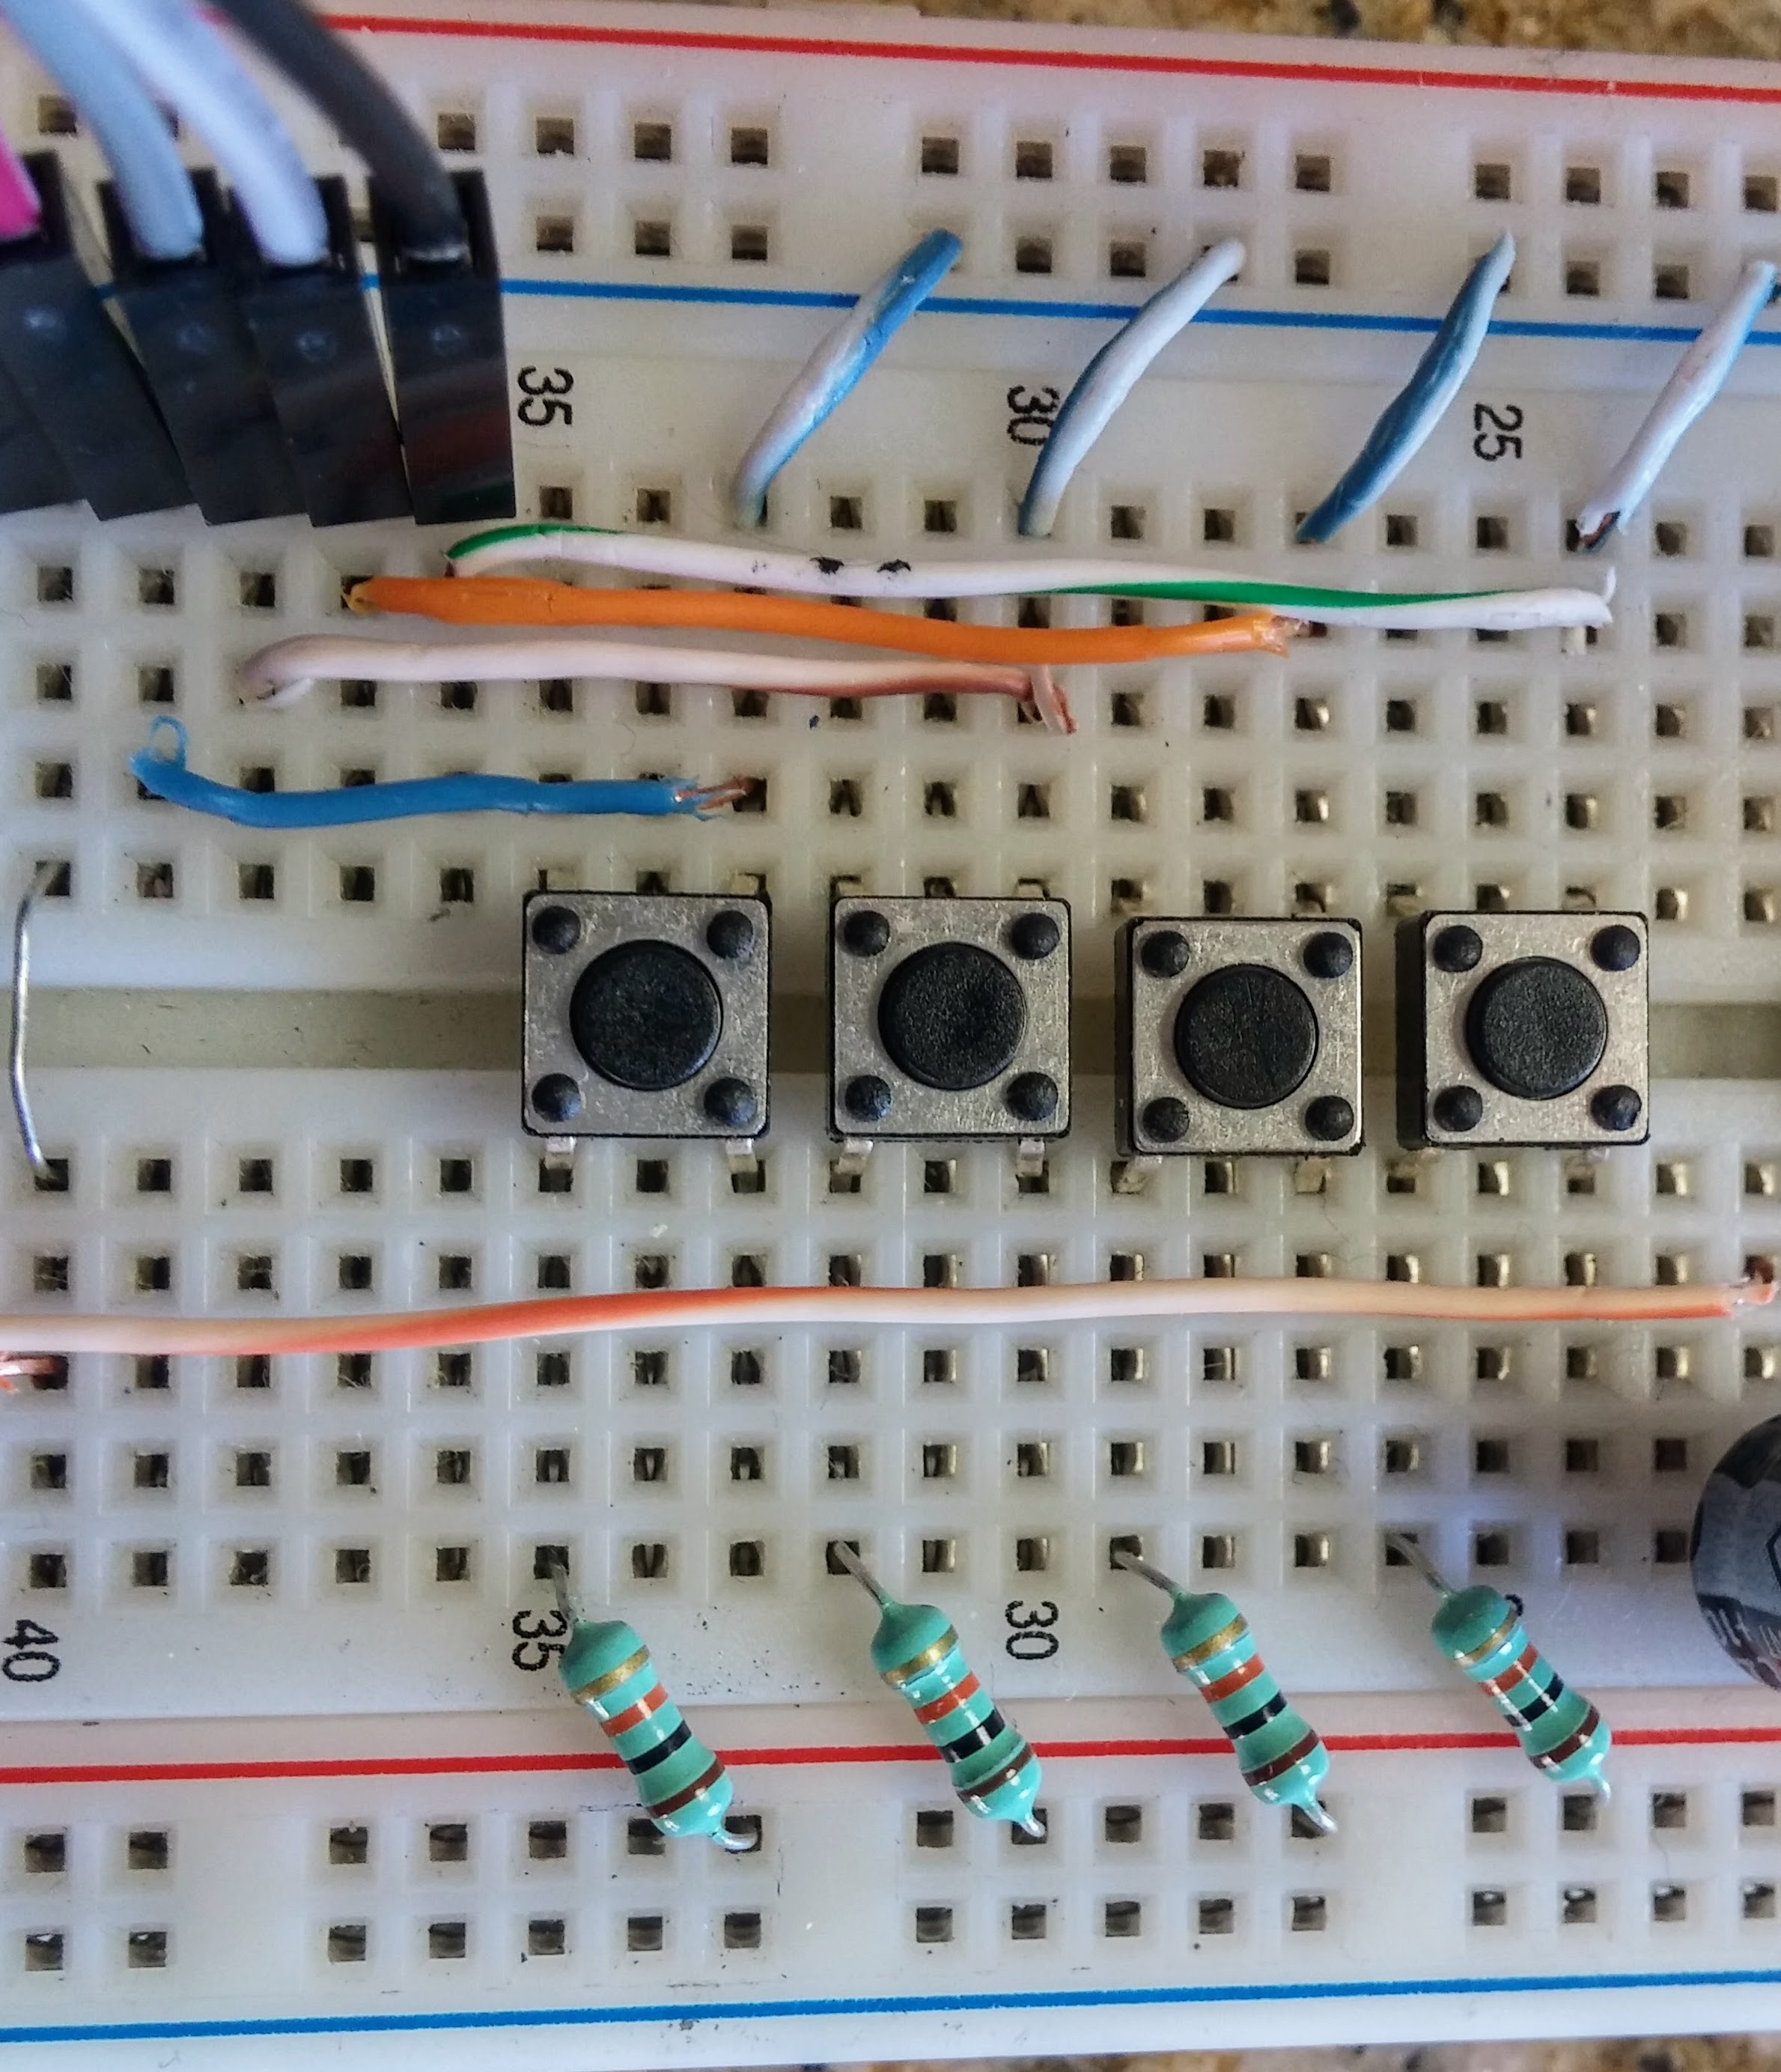
\includegraphics[width = 0.25\textwidth]{Switches_foto}}
\caption{Conexión de botones.}
\label{fig:pushbutton}
\end{figure}

\item \textbf{Conexión de convertidor digital-analógico.}\\
Se hacen las conexiones del convertidor digital-analógico (DAC) tal como se muestra en la figura \ref{fig:dac}.

\begin{figure}[H]
\centering
\subfigure[Diagrama]{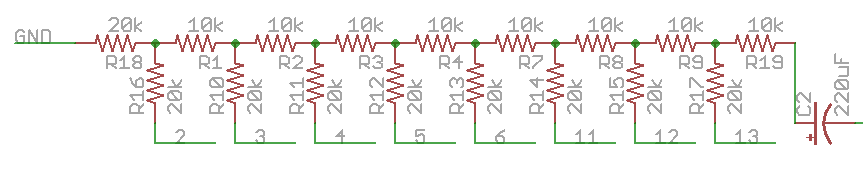
\includegraphics[width = 0.8\textwidth]{DAC}} \\
\subfigure[Ensamble en protoboard]{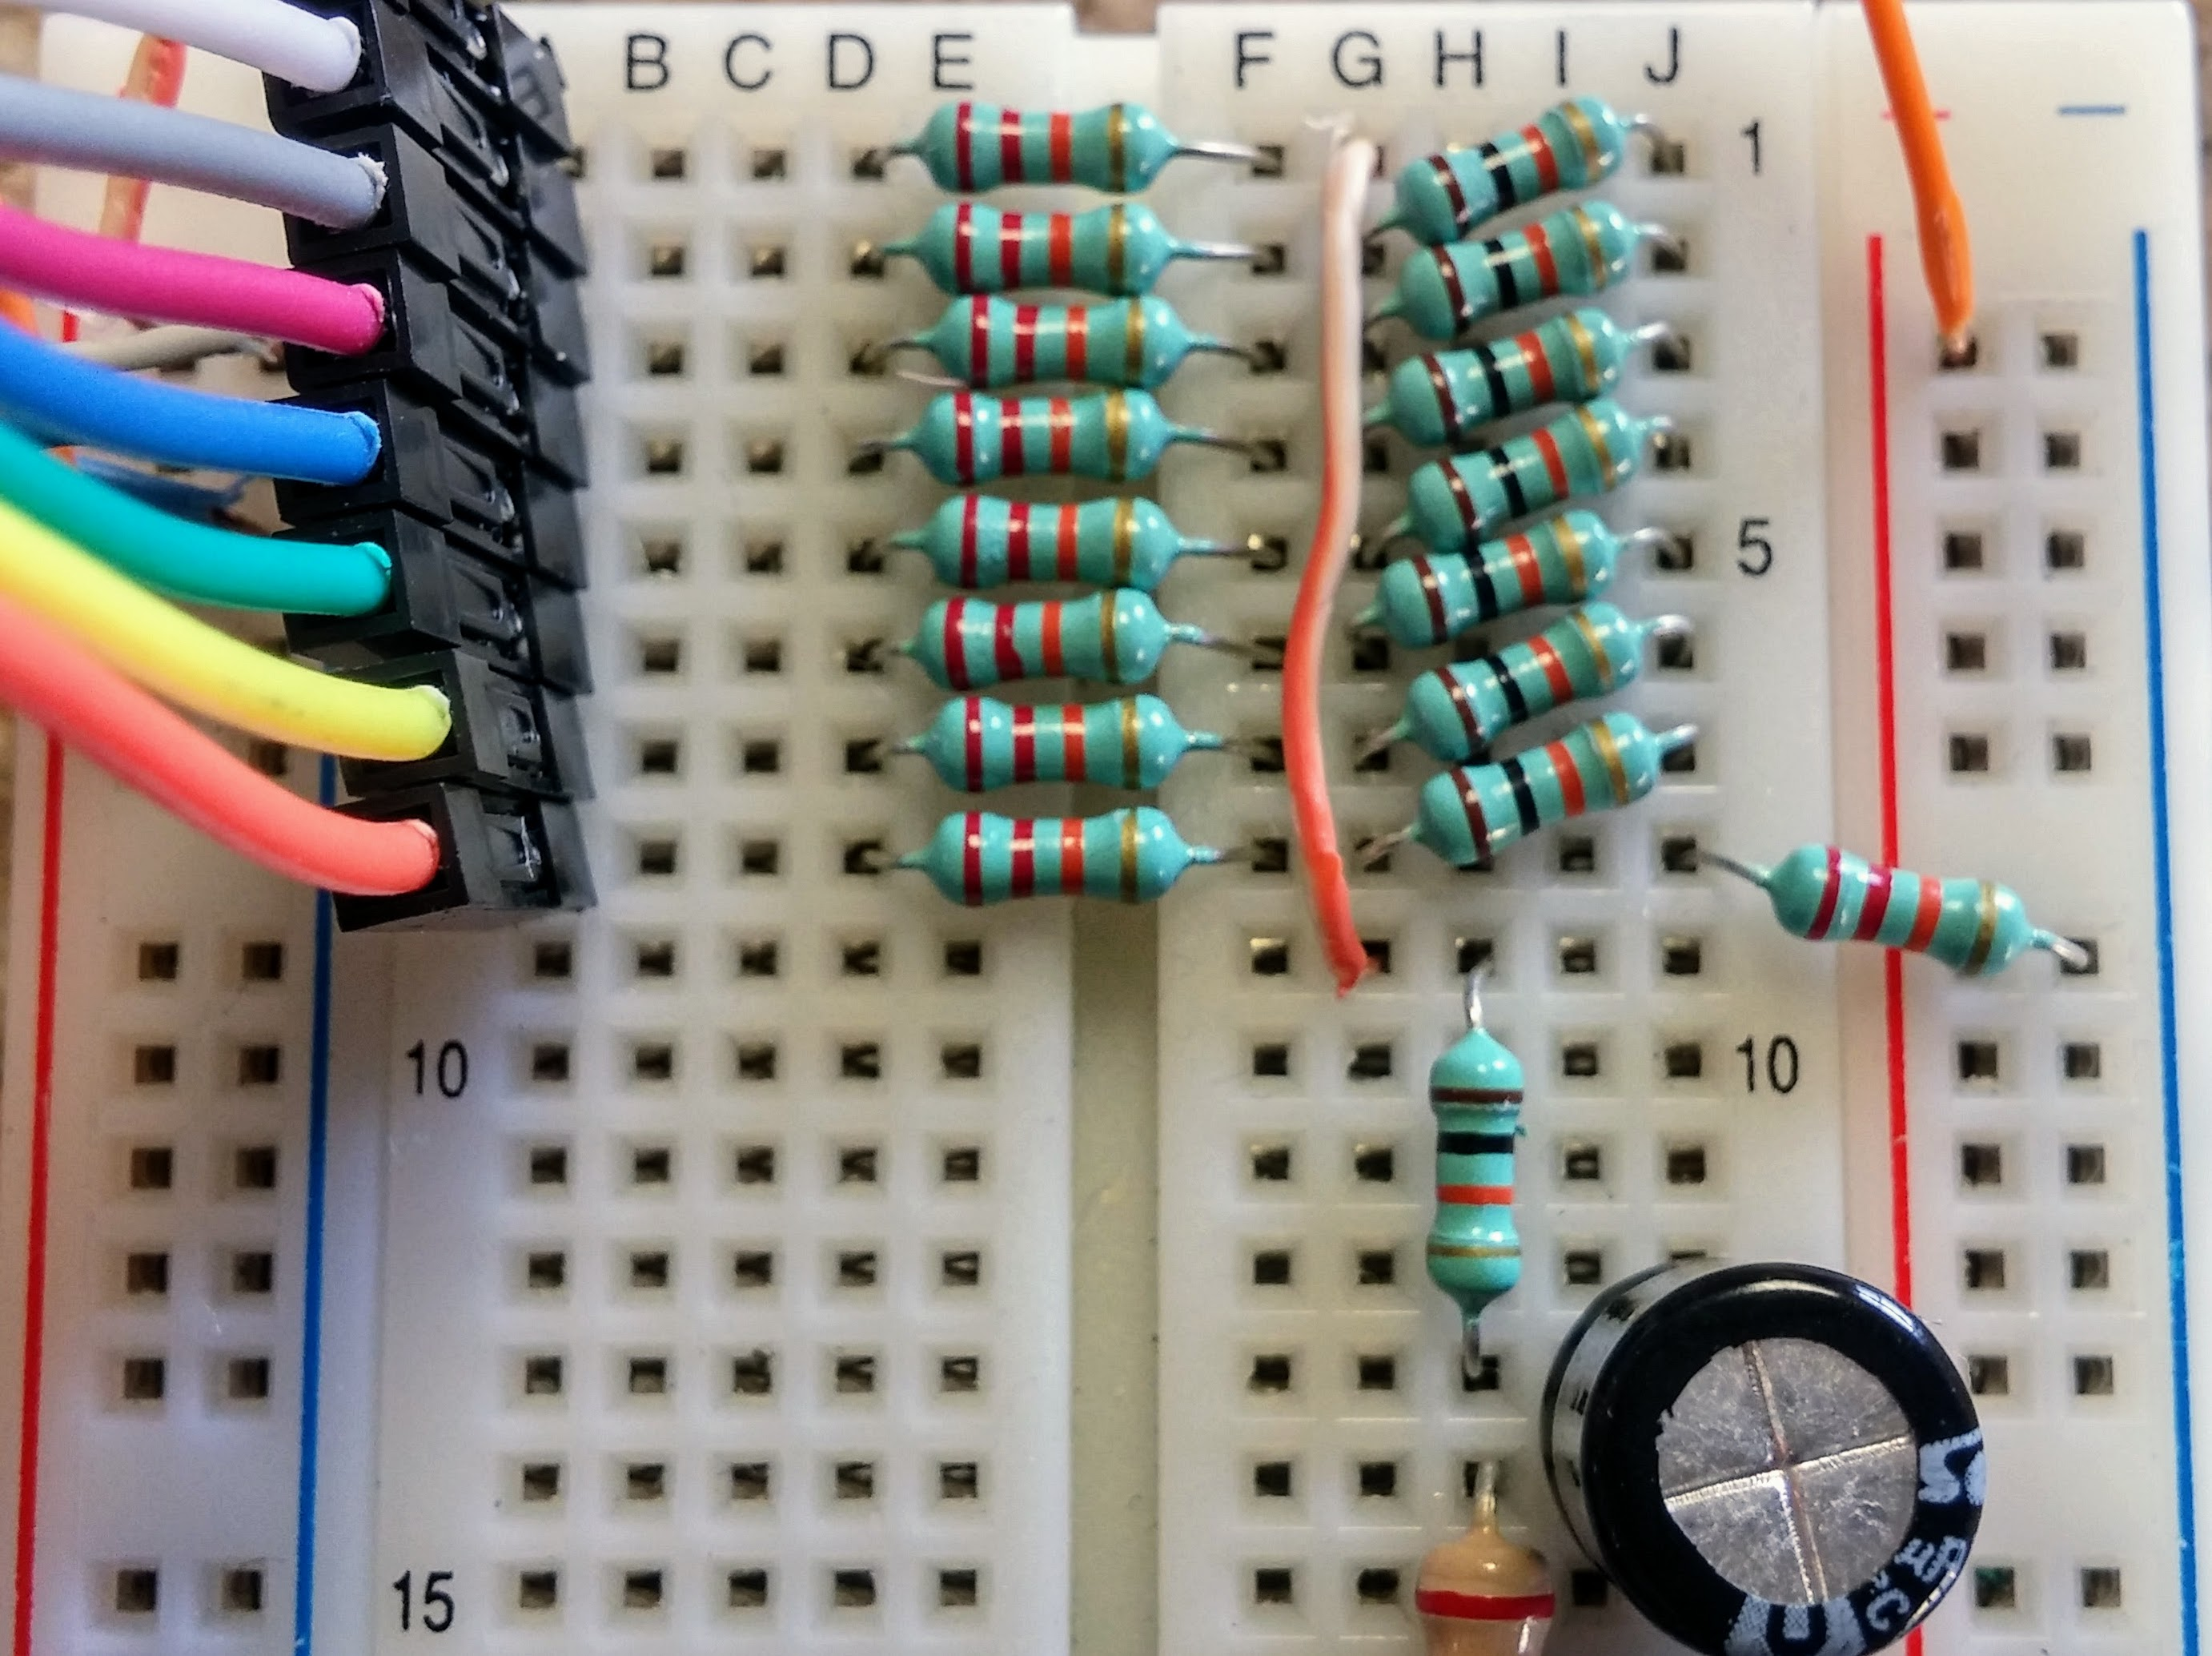
\includegraphics[width = 0.39\textwidth]{DAC_foto}}
\caption{Conexión del convertidor digital-analógico.}
\label{fig:dac}
\end{figure}

Para esto se conectan primero ocho resistores de 20k Ohms al protoboard, éstos deberán ir conectados a los pines digitales D0-D7 del Arduino. Después, se conectan 7 resistores de 10k Ohms, uno entre cada par de 20k Ohms. Un resistor de 20k Ohms se conecta a tierra y a la resistencia de 20k Ohms del pin D0. Por último, se conecta un resistor de 10k Ohms y un capacitor de 220$\mu$F a la resistencia de 20k Ohms del pin D7.


\item \textbf{Amplificador}

Primero se conecta el circuito integrado LM386N en el protoboard como se muestra en la figura \ref{fig:amp}. Se conecta un resistor de 20k Ohms a la terminal negativa del capacitor de 220$\mu$F al final del DAC y al pin 3 del LM356N.  El mismo pin también se conecta a tierra con resistor de 2.2k Ohms. Los pines 2 y 4 se conectan directamente a tierra. El pin 6 de alimentación se conecta a la fuente de 9V y el pin 5 de salida se conecta a un capacitor de 220$\mu$F.

\begin{figure}[htb]
\centering
\subfigure[Diagrama]{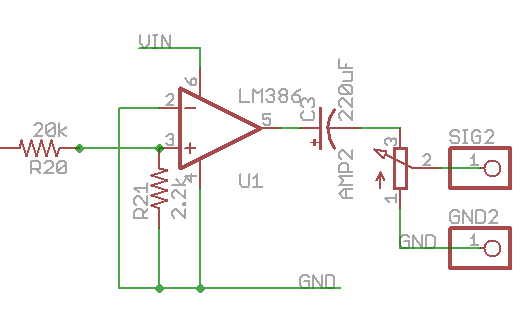
\includegraphics[width = 0.47\textwidth]{Amplificador}}
\subfigure[Ensamble en protoboard]{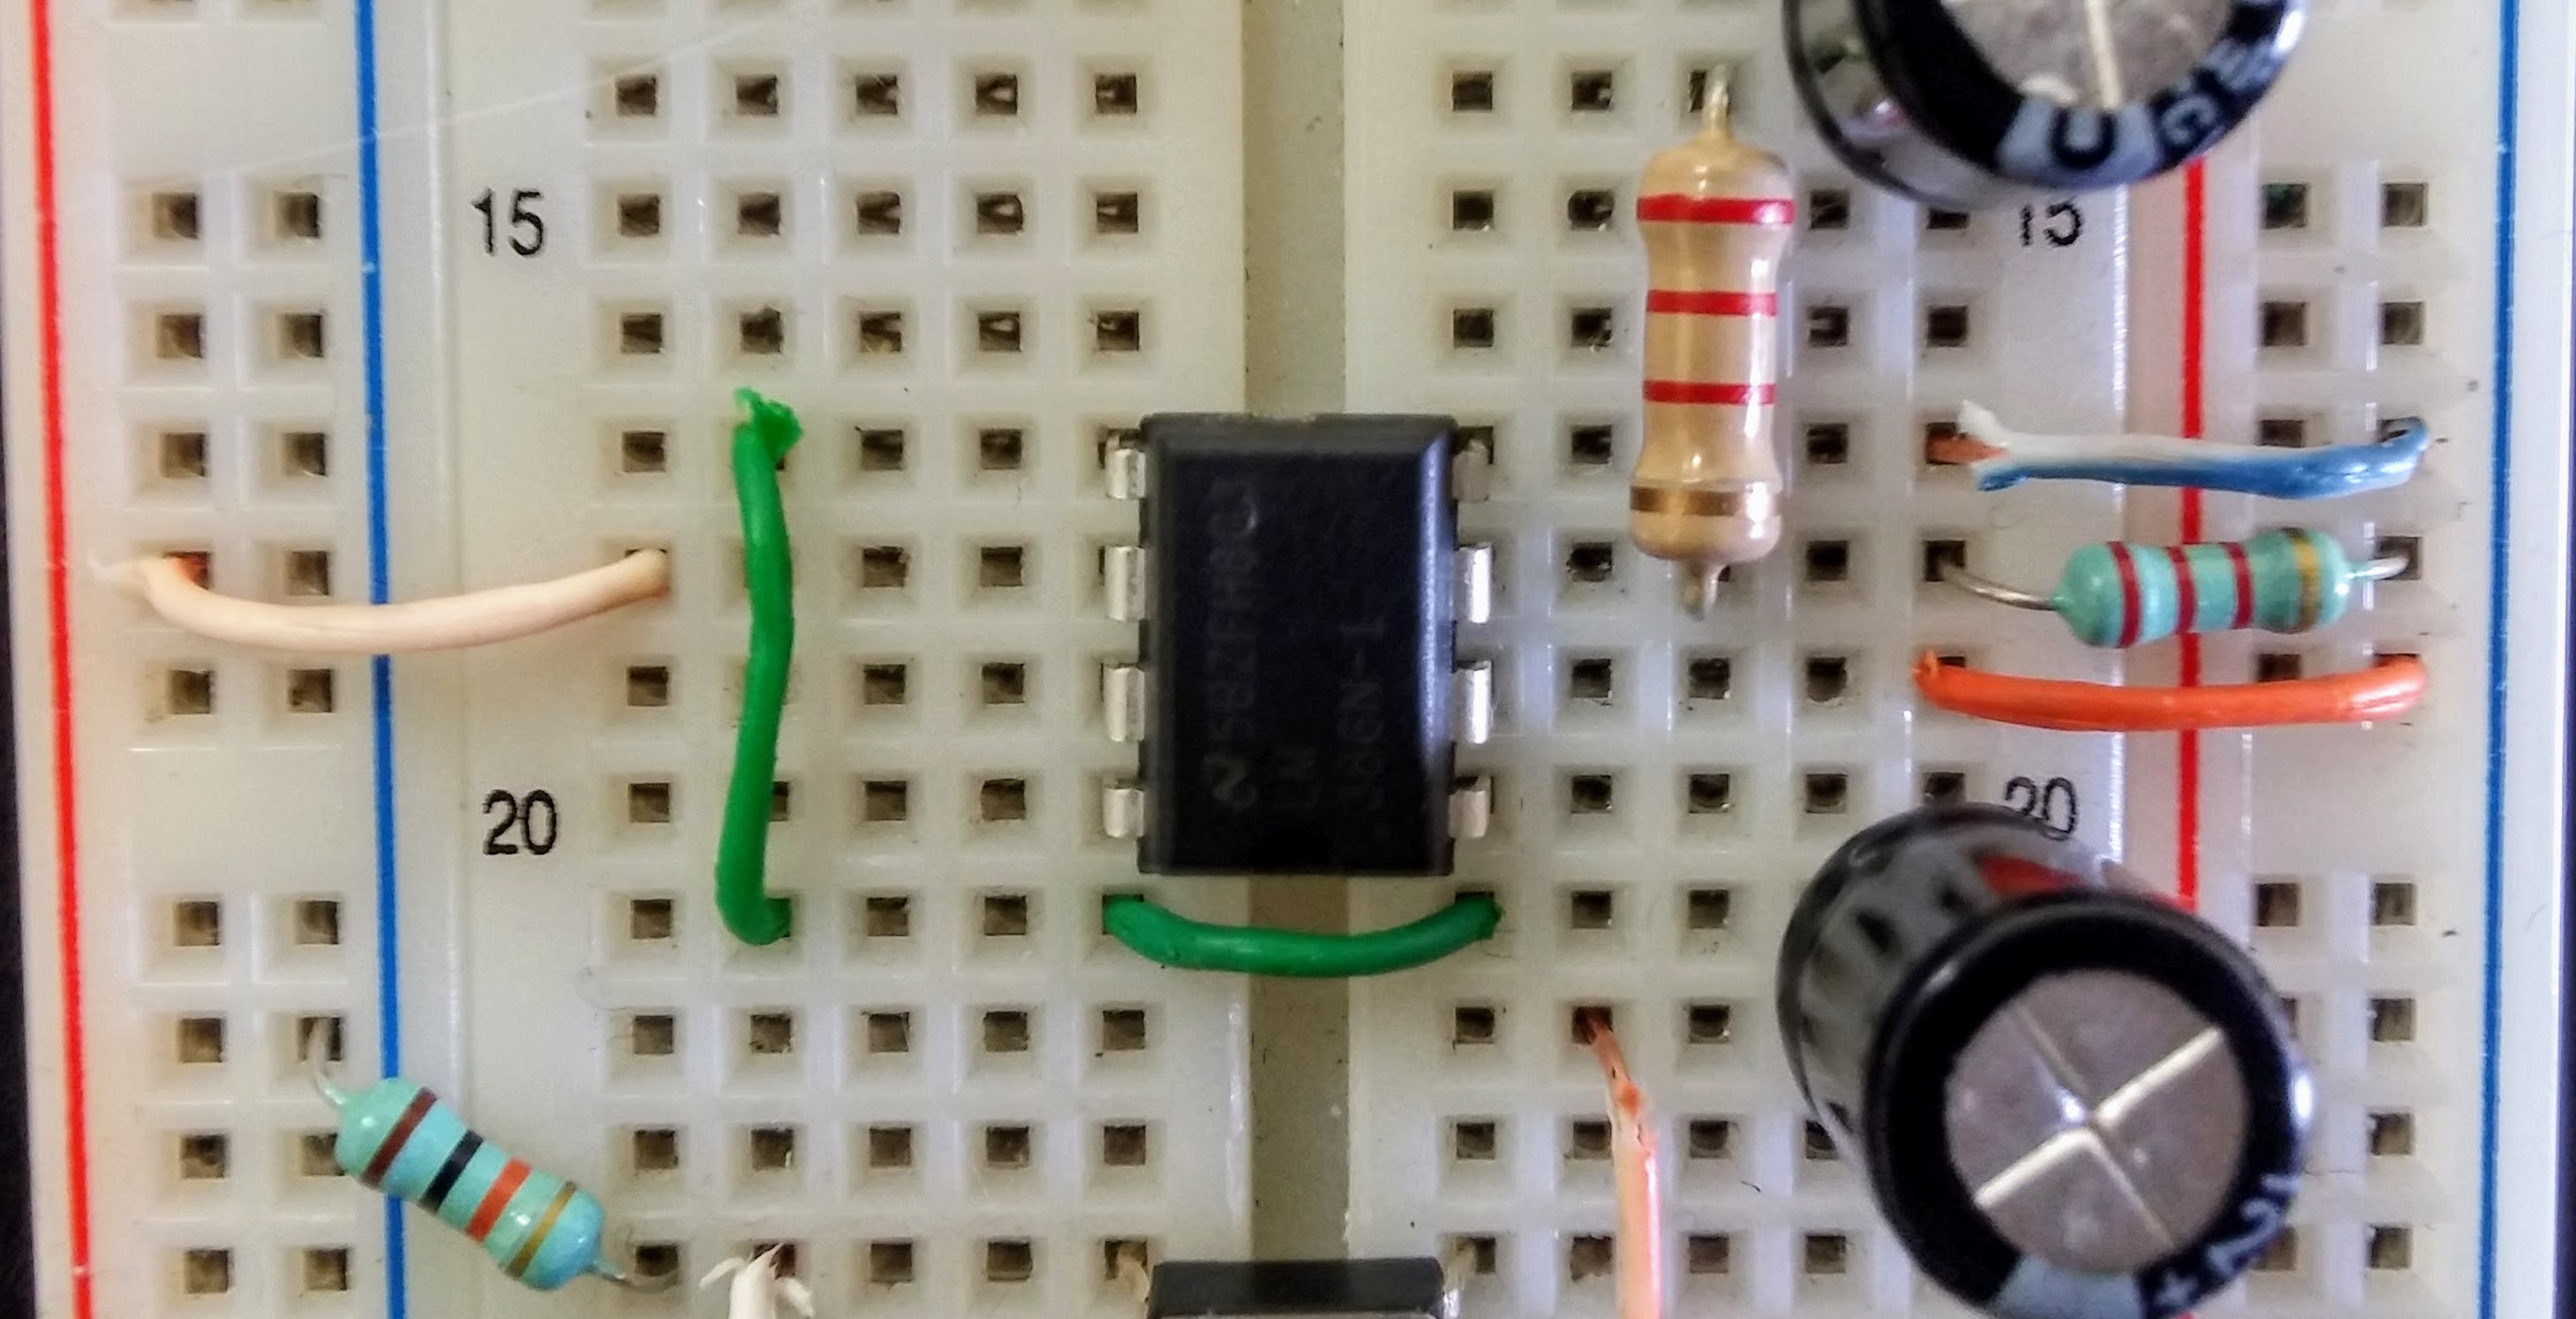
\includegraphics[width = 0.47\textwidth]{Amplificador_foto}}
\caption{Conexión del amplificador de señal}
\label{fig:amp}
\end{figure}


\item \textbf{Potenciómetros de frecuencia y PWM y ganancia}

Se conectan en el protoboard un potenciometro de 10k Ohms para la ganancia, uno de 50k Ohms para la frecuencia y otro 10k Ohms para el PWM, como se muestra en la figura \ref{fig:POTs}. El potenciómetro de ganancia se conecta al amplificador de señal como se muestra en el diagrama de la figura \ref{fig:amp}, con la terminal negativa del capacitor de 220$\mu$F en su pin derecho, la tierra en su pin izquierdo y la salida de señal en el pin central. Los potenciómetros de frecuencia y PWM se conectan, con sus pins derechos, al pin de 5V del Arduino, a tierra con sus pins izquierdos y los pins centrales van a las entradas analógicas A4 y A5 del Arduino.


\begin{figure}[H]
\centering
\subfigure[Diagrama para frecuencia y PWM]{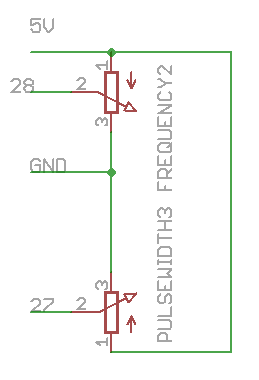
\includegraphics[width = 0.2\textwidth]{POT-PW-Freq}}
\subfigure[Ensamble en protoboard de ganancia (izq), frecuencia (cen) y PWM (der).]{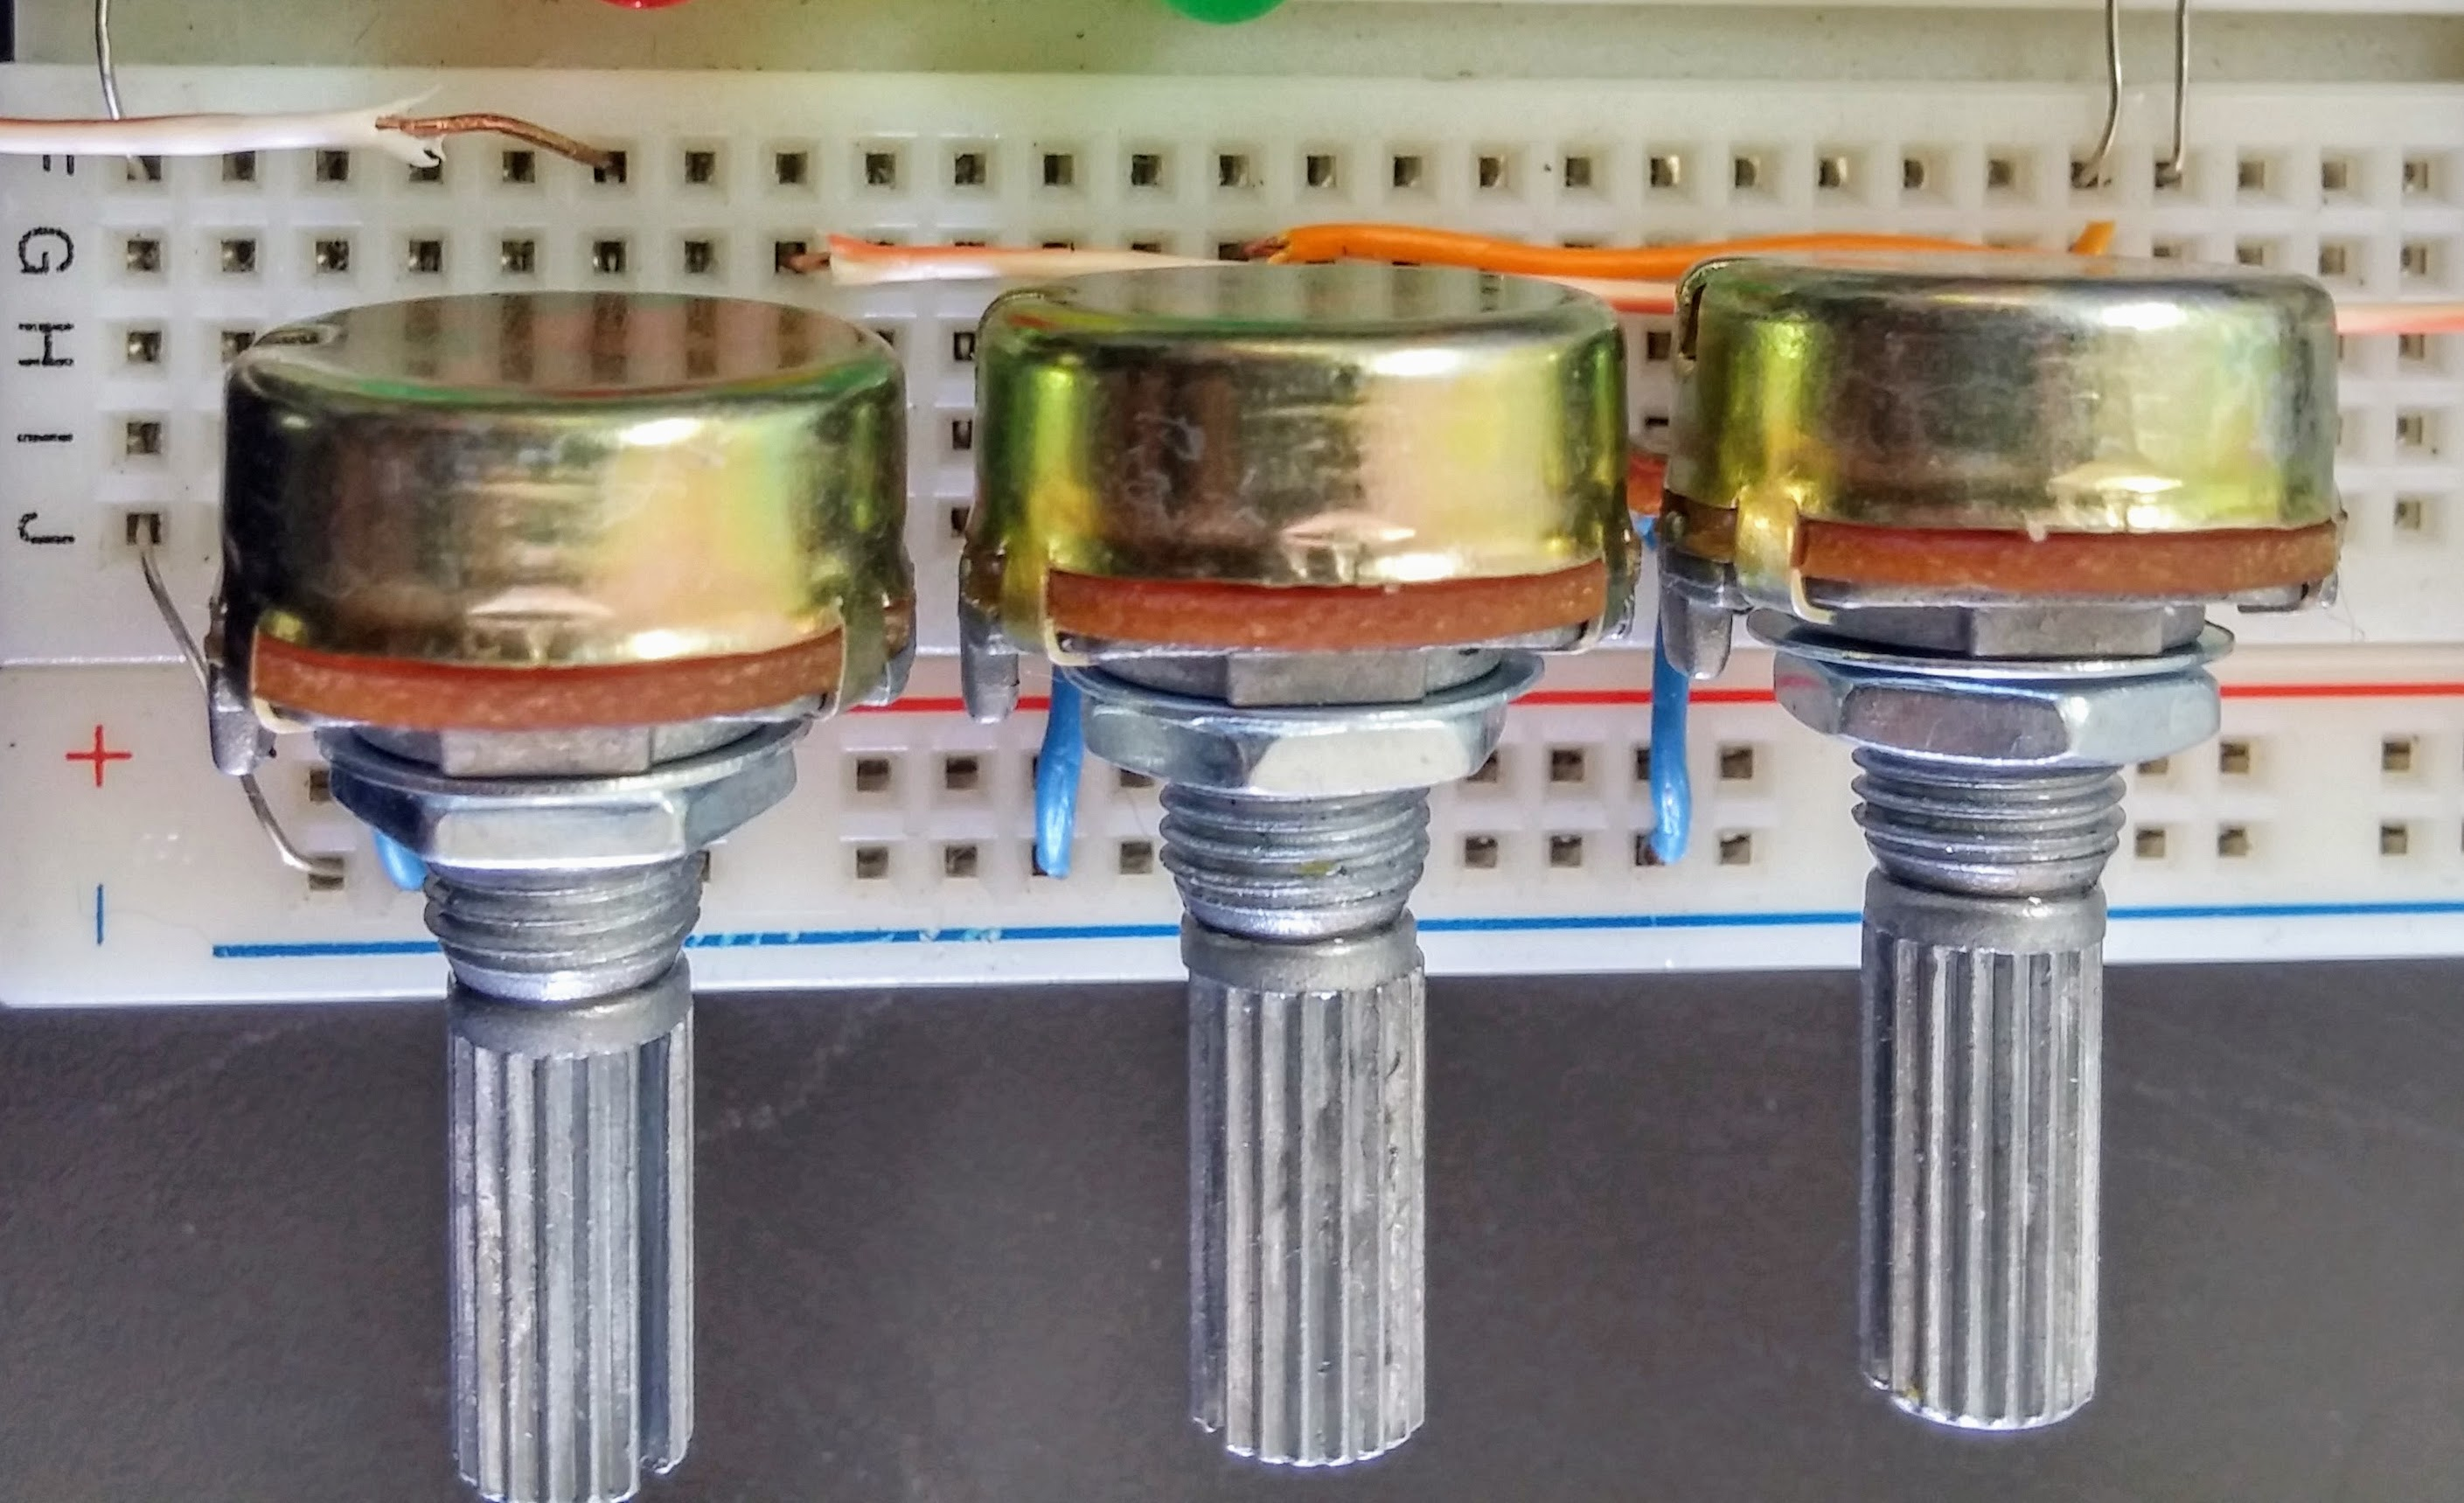
\includegraphics[width = 0.4\textwidth]{POT_foto}}
\caption{Conexión de potenciómetros.}
\label{fig:POTs}
\end{figure}


\item \textbf{Conexión de LEDs}
Se conectan 4 LEDs al protoboard como se muestra en la figura \ref{fig:leds}. Los cátodos se conectan a tierra con un resistor de 1k Ohm cada uno. Los ánodos se conectan a las salidas digitales D8-D11 del Arduino tomando en cuenta el siguiente orden:

\begin{itemize}
\item D8 = Pulso
\item D9 = Triangulo
\item D10 = Sierra
\item D11 = Seno
\end{itemize}

\begin{figure}[H]
\centering
\subfigure[Diagrama de LEDs.]{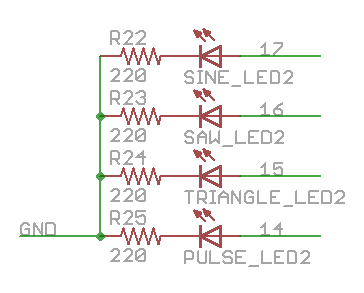
\includegraphics[width = 0.4\textwidth]{LED}}
\subfigure[Ensamble en protoboard.]{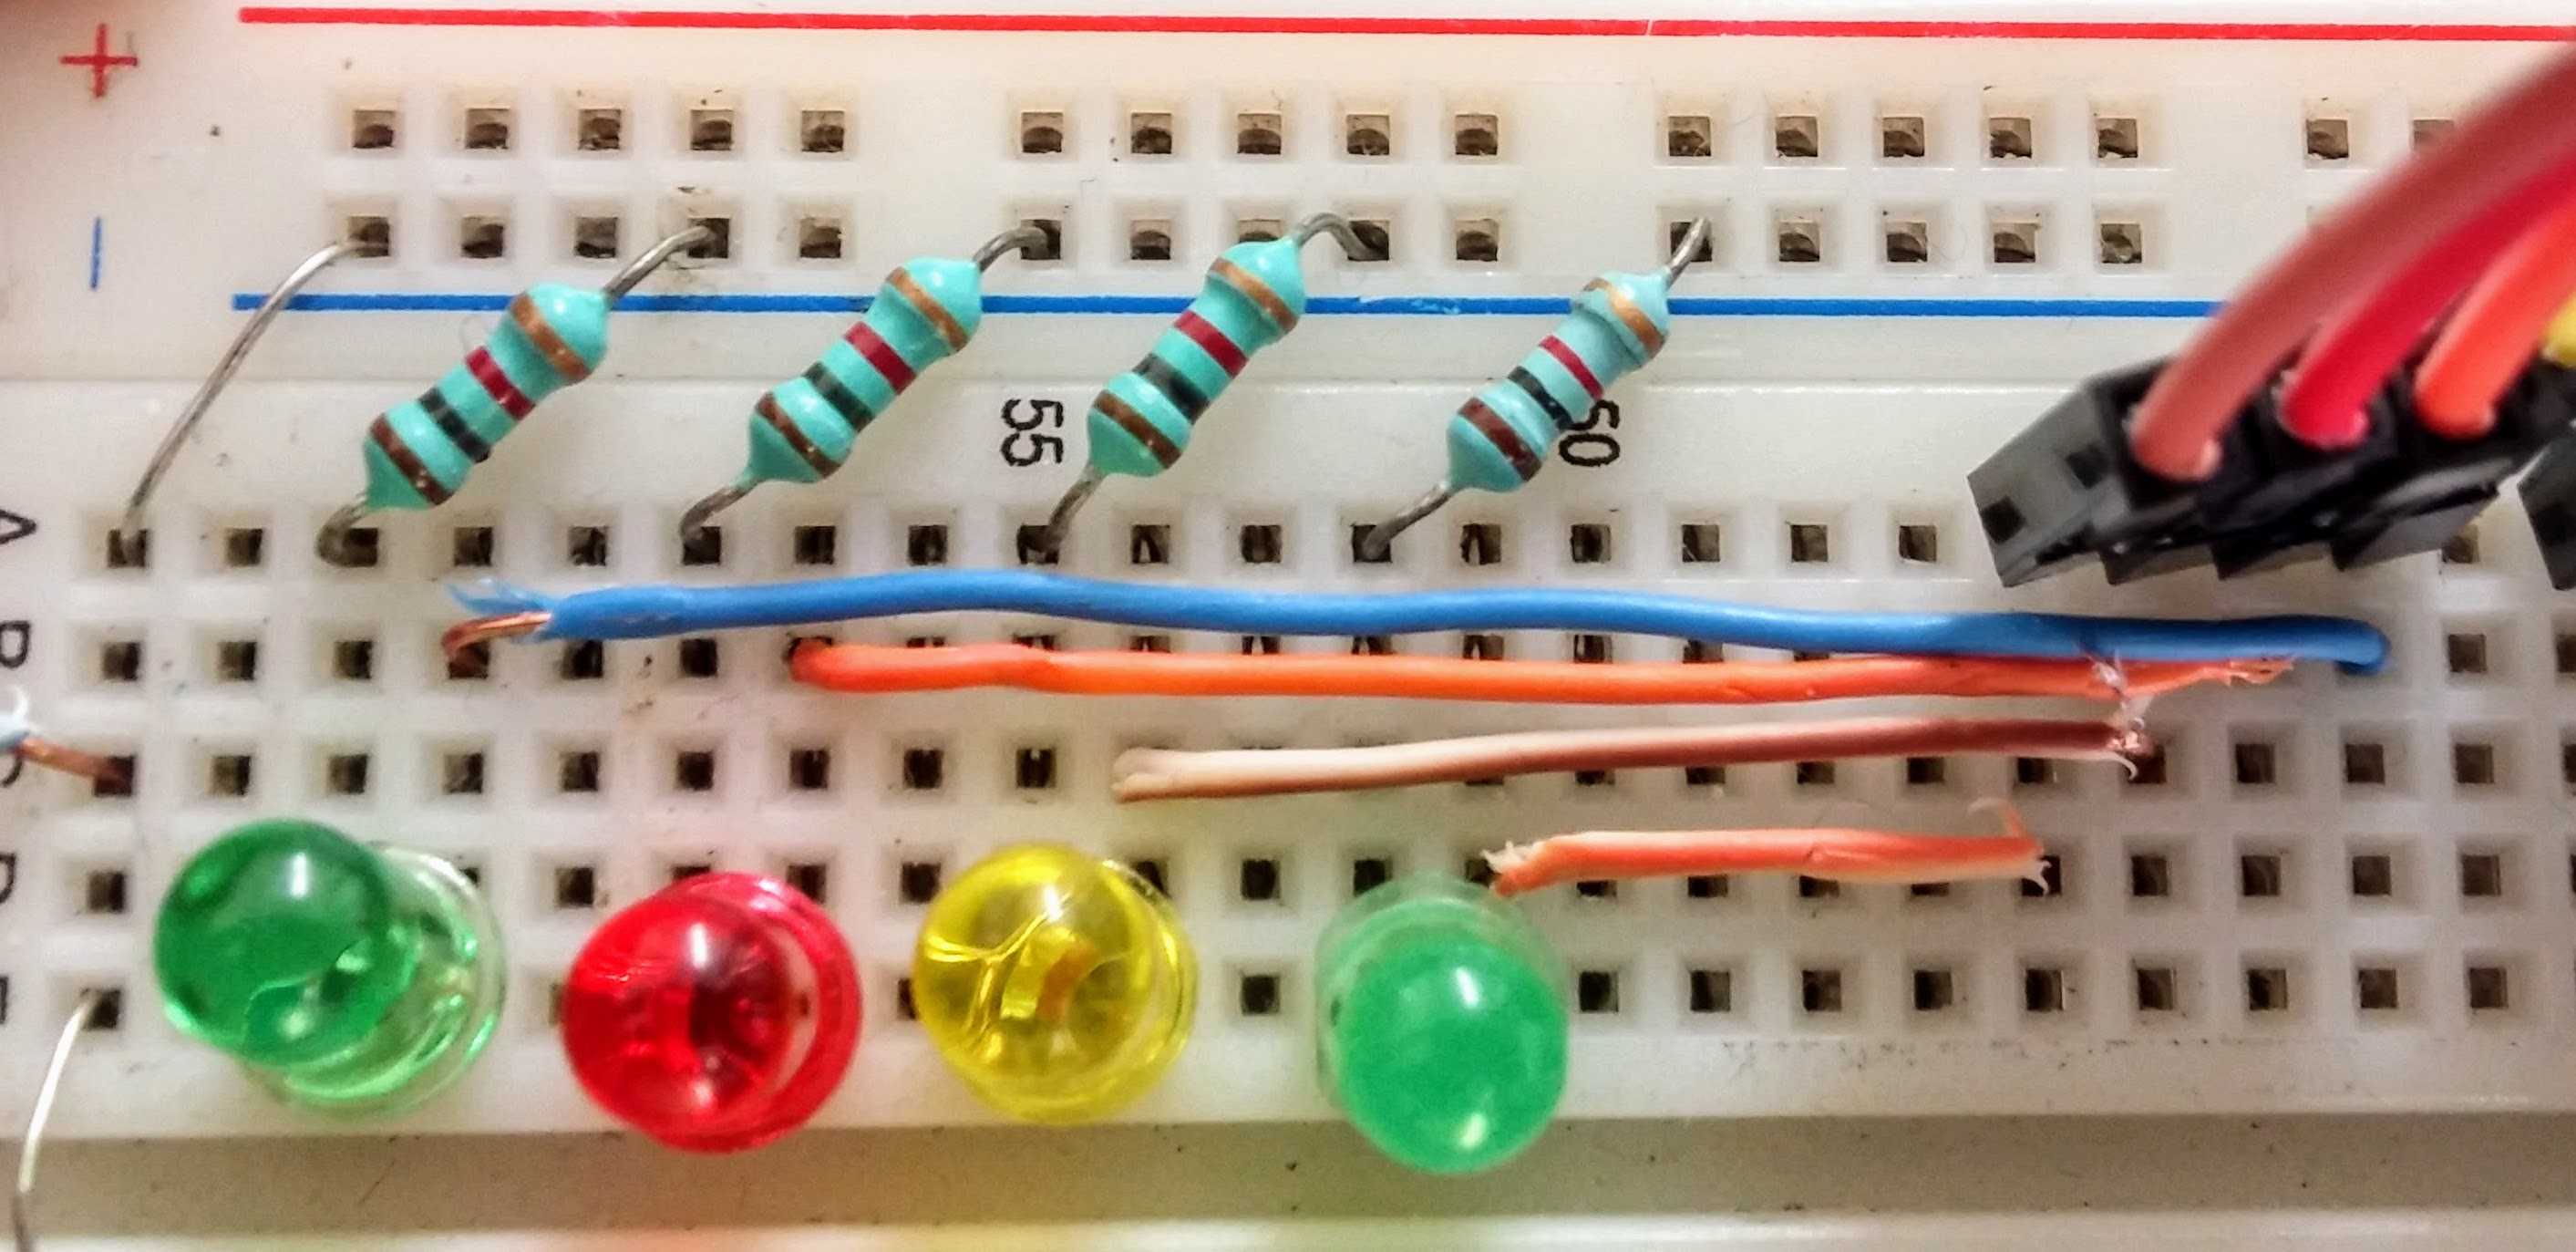
\includegraphics[width = 0.45\textwidth]{LEDS_foto}}
\caption{Conexión de LEDs}
\label{fig:leds}
\end{figure}

\item \textbf{Firmware}
El código \ref{alg:code} utilizado con el Arduino se muestra en el apéndice con comentarios que explican las secciones del mismo. Este código es una versión modificada del programa desarrollado por Amanda Ghassaei en abril del 2012. 
El código trabaja revisando primero el estado de los botones para así determinar que tipo de función generar. Después, lee las entradas analógicas de los potenciómetros para calcular la frecuencia que debe tener la señal y, en caso de hacer seleccionado la función cuadrada, el ancho de cada pulso. Una vez leídos estos parámetros, se procede a generar la función seleccionada y a enviarla a través de el puerto digital B (pins D0-D7).


\item \textbf{Circuito completo}
A continuación se muestra en la figura un diagrama completo de todo el circuito y como se ve este ya armado en el protoboard.

\begin{figure}[H]
\centering
\subfigure[Diagrama completo]{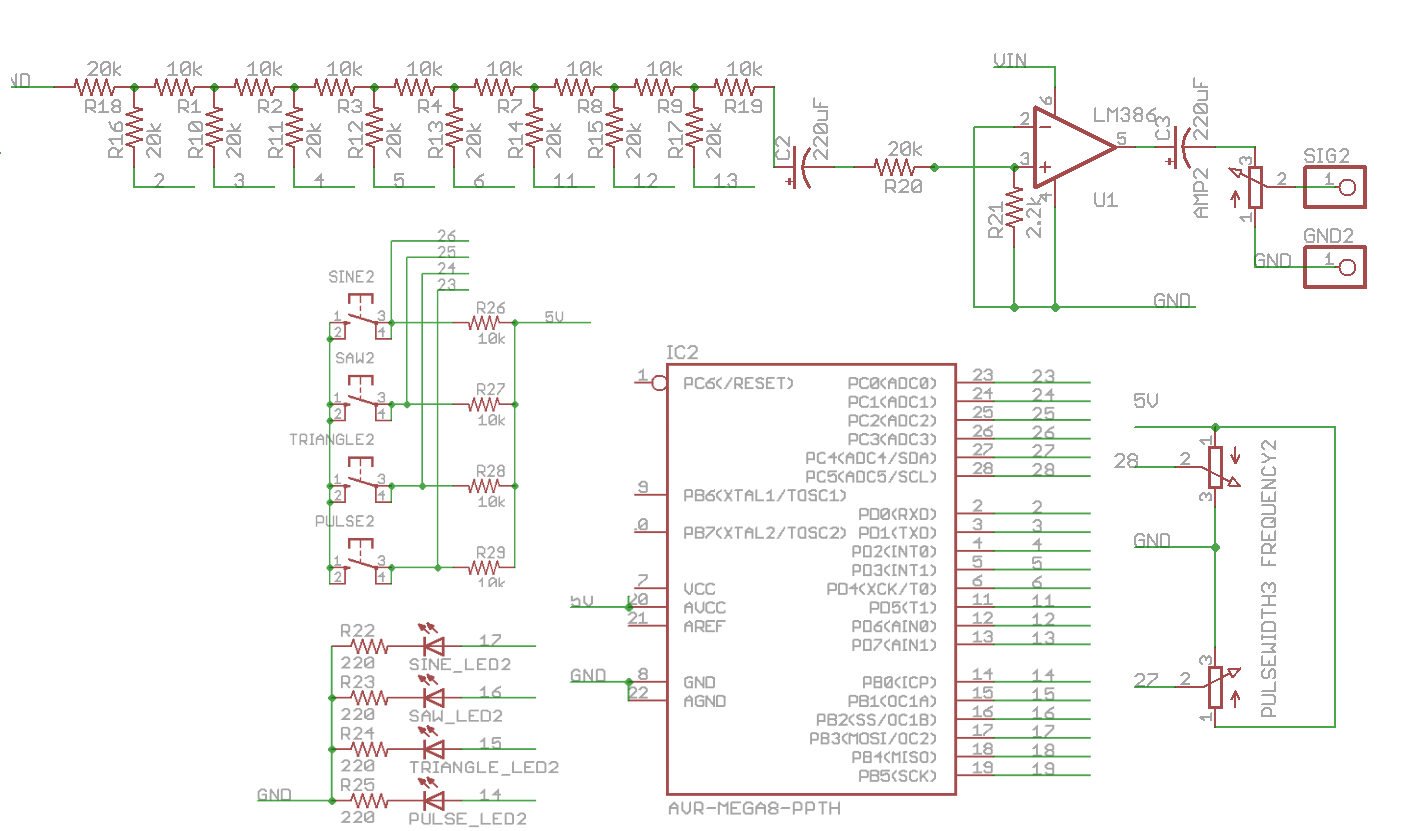
\includegraphics[width = 0.7\textwidth]{circuito}}
\subfigure[Ensamble completo]{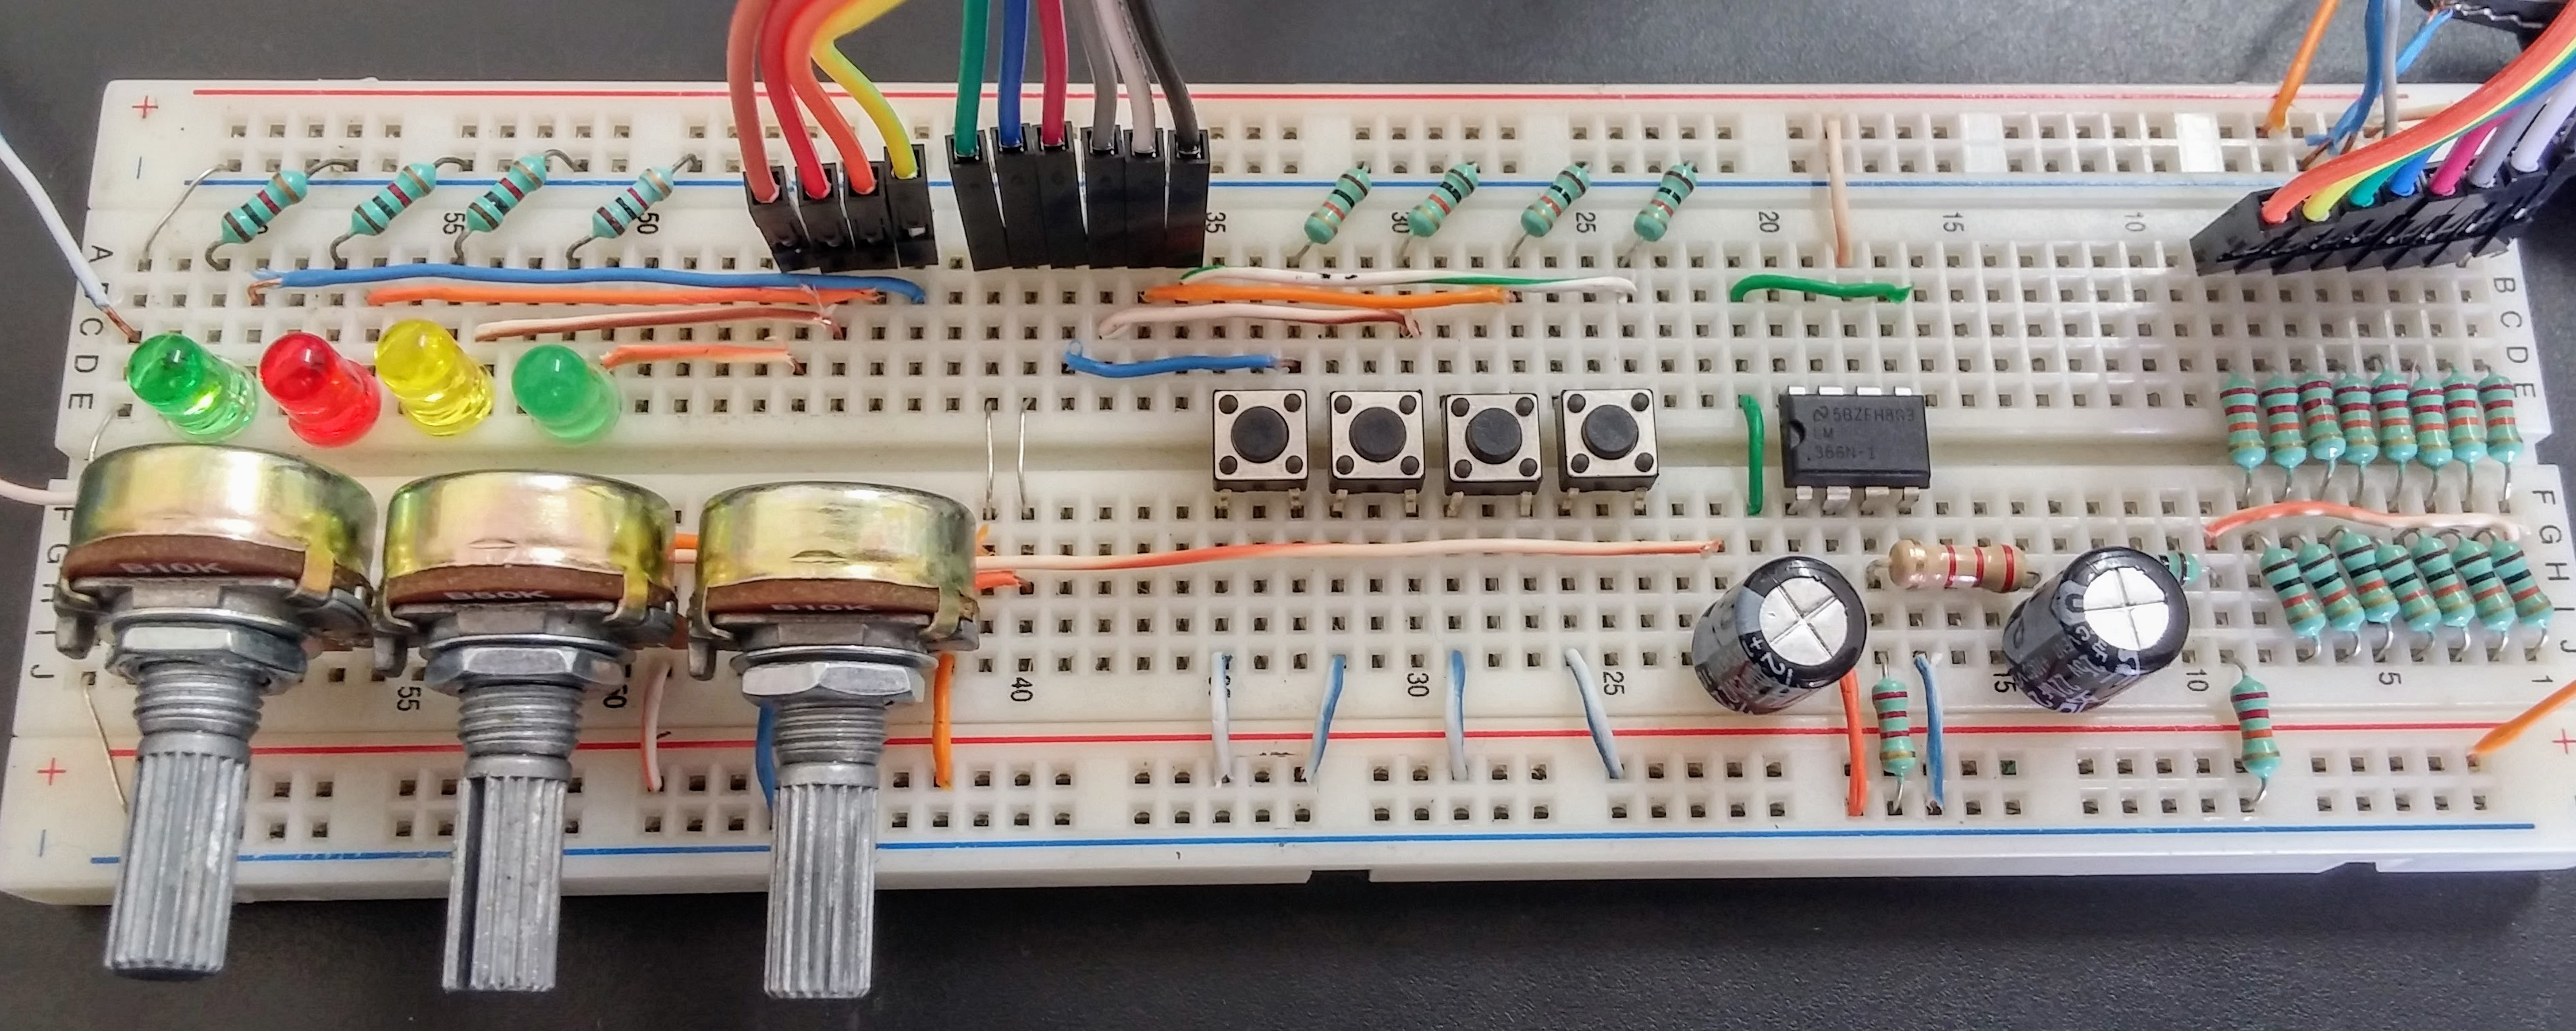
\includegraphics[width = 0.7\textwidth]{Completo}}
\caption{Generador de funciones terminado}
\label{fig:arduino}
\end{figure}
\end{enumerate}





\section{Conclusiones}
Se comprueba la importancia de la instrumentación en el proceso de realizar este proyecto pues al encontrarnos con dificultades técnicas, como que no se podía cambiar de tipo de onda al oprimir los botones, que la señal obtenida no parecía haber sido amplificada o que los potenciómetros no operaban bien al no incrementar ni disminuir los parámetros que debían de cambiar, la manera de llegar a una solución fue la de comprender bien el funcionamiento de cada componente y mediante un multímetro comprobar las conexiones y los voltajes correspondientes para cada parte del circuito.

En general, se concluye que este proyecto fue útil para reforzar y comprender conceptos de electrónica así como las habilidades manuales necesarias para la conexión de circuitos. Otro punto importante es que se aprendió como utilizar el microcontrolador Arduino, el cual resulta ser una plataforma versátil, cómoda y con gran aplicación educativa para introducir a los alumnos, como nosotros, a la electrónica y la instrumentación; Sin duda, estos conocimientos podrán ser útiles para futuros proyectos.

\bibliographystyle{unsrt}
\bibliography{ref}

\clearpage
\newpage
\section*{APÉNDICE}
\noindent
\textbf{NOTA:} En la linea 34 faltan valores en la definición de sine20000, para el código completo visite: \\
\url{https://github.com/HiramHerrera/Wave-Function-Generator}
\begin{lstlisting}[language=C, caption=Código implementado para el generador de funciones, label = alg:code]
//Arduino Function Generator
//by Amanda Ghassaei
//http://www.instructables.com/id/Arduino-Waveform-Generator/
//April 2012
//
//Modified by: Hiram Herrera & Osvaldo Rosales
//May 2017

/*
 * This program is free software; you can redistribute it and/or modify
 * it under the terms of the GNU General Public License as published by
 * the Free Software Foundation; either version 3 of the License, or
 * (at your option) any later version.
 *
*/

//in most of this code I have used the arduino portpin assignments to send data to pins, you can read more about how that works here: http://www.arduino.cc/en/Reference/PortManipulation

/*********************************************************
some notes about pin setup:
4 momentary switches control waveshape (analog in 0-3)
   -sine connects to A0
   -triangle A1
   -saw A2
   -pulse A3
freq control pot (log taper) is connected to analog in 4
pulse width modulation pot (linear taper) connected to anolog in 5
PORT D (digital pins 0-7) are 8 bit function out
PORT B (digital pins 8-13) are 8 bit function out

*********************************************************/

//Storing sine wave values in size 20000 array
const byte sine20000[] PROGMEM = {127, 127, ...,}
//Defining variables
//wavetype storage:
//0 is pulse
//1 is triangle
//2 is saw
//3 is sine
byte type = 1;//initialize as square
byte typecurrent = 0;
byte typelast;
byte typecounter[4];
byte i;

//variables for PW pot monitoring
float pulseWidth;
int pulseWidthScaled;
int PWCurrent;
byte PWTolerance = 8;//adjust this to increase/decrease stability of PW measurement

//variables for freq pot monitoring
int frequency;
int freqCurrent;
byte freqTolerance = 2;//adjust this to increase/decrease stability of frequency measurement
unsigned int freqscaled;

byte wave;
long t;
long samplerate;
long period;

//storage variables- I used these to cut down on the math being performed during the interrupt
int sawByte = 0;
byte sawInc;
int triByte = 0;
byte triInc;
int sinNum = 0;
int sinInc;

void setup() {
  
  //set port/pin  mode
  DDRD = 0xFF;//all outputs
  DDRC = 0x00;//all inputs
  DDRB = 0xFF;//all outputs
  //TIMER INTERRUPT SETUP
  
  cli();//disable interrupts
  //timer 1:
  TCCR1A = 0;// set entire TCCR1A register to 0
  TCCR1B = 0;// same for TCCR1B
  //set compare match register- 100khz to start
  OCR1A = 159; // = (16 000 000 / 100 000) - 1 = 159
  //turn on CTC mode
  TCCR1B |= (1 << WGM12);
  // Set CS10 bit for 0 prescaler
  TCCR1B |= (1 << CS10);
  // enable timer compare interrupt
  TIMSK1 |= (1 << OCIE1A); 
  
  samplerate = 100000;
  
  PORTB = 0;
  PORTB = 1<<type; //Send signal value to PORTB
  
  //initialize variables
  frequency = analogRead(A5);//initialize frequency
  freqscaled = 48*frequency+1;//from 1 to ~50,000\
  period = samplerate/freqscaled;
   
  pulseWidth = analogRead(A4);//initalize pulse width
  pulseWidthScaled = int(pulseWidth/1023*period);

  //Number of steps for each wave
  triInc = 511/period;
  sawInc = 255/period;
  sinInc = 20000/period;
  
  sei();//enable interrupts
}

void checkFreq() {
  freqCurrent = analogRead(A5);
  if (abs(freqCurrent-frequency)>freqTolerance){//if reading from pot exceeds tolerance
    frequency = freqCurrent;//new frequency- number between 0 and 1024
    freqscaled = 48*frequency+1;//from 1 to ~50,000Hz
    period = samplerate/freqscaled;
    pulseWidthScaled = int(pulseWidth/1023*period);
    triInc = 511/period;
    if (triInc==0){
      triInc = 1;
    }
    sawInc = 255/period;
    if (sawInc==0){
      sawInc = 1;
    }
    sinInc=20000/period;
  }
}

void checkPW() {
  PWCurrent = analogRead(A4);
  if (abs(PWCurrent-pulseWidth)>PWTolerance){//if reading from pot exceeds tolerance
    pulseWidth = PWCurrent;//new pulse width, val between 0 and 1023
    pulseWidthScaled = int(pulseWidth/1023*period);
  }
}


void checkShape() {//check states of buttons
//  4 momentary switches control waveshape
//   -pulse connects to A0
//   -triangle A1
//   -saw A2
//   -sine A3
  typelast = typecurrent;
if (digitalRead(A0)==HIGH){
  typecurrent  = 1;
}
else if (digitalRead(A1)==HIGH){
  typecurrent = 2;
}
else if (digitalRead(A2)==HIGH){
  typecurrent = 4;
}
else if (digitalRead(A3)==HIGH){
  typecurrent = 8;
}
//This part allows momentary switches to work properly
  for (i=0; i<4; i++){
    if (i==type){
    }
    else{
      if ((typecurrent & (1 << i)) ^ (typelast & (1 << i))){//current diff than prev and debounce
        if ((typecurrent & (1 << i))){//currently depressed
            type = i;//set wave type
        }
        else {
          typecounter[i] = 12;//else set debounce counter to 12
        }
      }
      else if (((typecurrent & (1 << i)) == (typelast & (1 << i )))) {//if current same as prev and diff than debounce
        if (typecounter[i] > 0 && --typecounter[i] == 0) {//decrease debounce counter and check to see if = 0
          if ((typecurrent & (1 << i))){//if debounce counter = 0 toggle debounced state
            type = i;
          }
        }
      }
    }
  }
}
    
 

ISR(TIMER1_COMPA_vect){//timer 1 interrupt
  //increment t and reset each time it reaches period
  t += 1;
  if (t >= period){
    t = 0;
  }
  switch (type) {
    case 0://pulse
    if (pulseWidthScaled <= t) {
      wave = 255;
    }
    else{
      wave = 0;
    }
    break;
    case 1://triangle
    if((period-t) > t) {
      if (t == 0){
        triByte = 0;
      }
      else{
        triByte += triInc;
      }
    }
    else{
      triByte -= triInc;
    }
    if (triByte>255){
      triByte = 255;
    }
    else if (triByte<0){
      triByte = 0;
    }
    wave = triByte;
    break;
    case 2://saw
    if (t=0){
      sawByte=0;
    }
    else{
      sawByte+=sawInc;
    }
    wave = sawByte;
    break;
    case 3://sine
    sinNum = t*sinInc;
    wave = pgm_read_byte_near(sine20000 + sinNum);
    break;
  }

  PORTD = wave;
}

void loop() {
  checkFreq(); //Check frequency values from POT in A5
  checkShape();//Check wave selection - Values from pins A0-A3
  checkPW();   //Check Pulse Width from pin A4 in case wave shape is pulse
  PORTB = 1<<type; //Send value to PORTB
}
\end{lstlisting}
\end{document}












